\documentclass[12pt,a4]{article}\usepackage[]{graphicx}\usepackage[]{xcolor}
% maxwidth is the original width if it is less than linewidth
% otherwise use linewidth (to make sure the graphics do not exceed the margin)
\makeatletter
\def\maxwidth{ %
  \ifdim\Gin@nat@width>\linewidth
    \linewidth
  \else
    \Gin@nat@width
  \fi
}
\makeatother

\definecolor{fgcolor}{rgb}{0.345, 0.345, 0.345}
\newcommand{\hlnum}[1]{\textcolor[rgb]{0.686,0.059,0.569}{#1}}%
\newcommand{\hlstr}[1]{\textcolor[rgb]{0.192,0.494,0.8}{#1}}%
\newcommand{\hlcom}[1]{\textcolor[rgb]{0.678,0.584,0.686}{\textit{#1}}}%
\newcommand{\hlopt}[1]{\textcolor[rgb]{0,0,0}{#1}}%
\newcommand{\hlstd}[1]{\textcolor[rgb]{0.345,0.345,0.345}{#1}}%
\newcommand{\hlkwa}[1]{\textcolor[rgb]{0.161,0.373,0.58}{\textbf{#1}}}%
\newcommand{\hlkwb}[1]{\textcolor[rgb]{0.69,0.353,0.396}{#1}}%
\newcommand{\hlkwc}[1]{\textcolor[rgb]{0.333,0.667,0.333}{#1}}%
\newcommand{\hlkwd}[1]{\textcolor[rgb]{0.737,0.353,0.396}{\textbf{#1}}}%
\let\hlipl\hlkwb

\usepackage{framed}
\makeatletter
\newenvironment{kframe}{%
 \def\at@end@of@kframe{}%
 \ifinner\ifhmode%
  \def\at@end@of@kframe{\end{minipage}}%
  \begin{minipage}{\columnwidth}%
 \fi\fi%
 \def\FrameCommand##1{\hskip\@totalleftmargin \hskip-\fboxsep
 \colorbox{shadecolor}{##1}\hskip-\fboxsep
     % There is no \\@totalrightmargin, so:
     \hskip-\linewidth \hskip-\@totalleftmargin \hskip\columnwidth}%
 \MakeFramed {\advance\hsize-\width
   \@totalleftmargin\z@ \linewidth\hsize
   \@setminipage}}%
 {\par\unskip\endMakeFramed%
 \at@end@of@kframe}
\makeatother

\definecolor{shadecolor}{rgb}{.97, .97, .97}
\definecolor{messagecolor}{rgb}{0, 0, 0}
\definecolor{warningcolor}{rgb}{1, 0, 1}
\definecolor{errorcolor}{rgb}{1, 0, 0}
\newenvironment{knitrout}{}{} % an empty environment to be redefined in TeX

\usepackage{alltt}

% ---- Metadata ---- %

\title{Honesty by Convenience: Corruption Tolerance in Ecuador}
\author{Daniel Hernán Sánchez Pazmiño}
\date{June 2022}

% ---- Load Packages ---- %

% Math

\usepackage{savesym} % Need to "save" the command that is already defined \varTheta

\usepackage{amsmath}
  \savesymbol{varTheta} 

% Fonts

% To set the TNR font for both text and equations:

\usepackage{mathspec}
  \setallmainfonts(Digits,Greek,Latin){Times New Roman}
\restoresymbol{MTP}{varTheta}

% Formatting

\usepackage{setspace}
  \doublespacing

\usepackage[margin = 1in]{geometry}

\usepackage{lscape}

% Citation & Bibliographies

\usepackage[backend = biber, style = apa, citestyle = apa]{biblatex}
  \addbibresource{refs.bib}
  
% For tables:

 % For the modelsummary tables:
\usepackage{siunitx}
\usepackage{booktabs} 
  \newcolumntype{d}{S[input-symbols = ()]}

\usepackage{caption}
\usepackage{multirow}
\usepackage[flushleft]{threeparttable}
  
% Other packages

\usepackage{csquotes} % For quotation marks

\usepackage{epigraph} % For epigraph
  \setlength\epigraphwidth{9cm}
  \setlength\epigraphrule{1pt}

\usepackage{float} % For the H float option- only used in emergencies (lol)

\usepackage{textcomp} % For the registered trademark symbol.

% Always load these packages at the end of the preamble:

\usepackage{hyperref}

% ---- R Stuff to be used in the whole document ----

% Here I will execute or source R code through chunks that I need to use throughout the whole document.

% General settings



% Load the data by sourcing the data manipulation script. Note that survey design objects are indeed created in this script.


\IfFileExists{upquote.sty}{\usepackage{upquote}}{}
\begin{document}
\maketitle
\clearpage

% ---- Sections ---- %

% Abstract Child Document


% Abstract .Rnw File


\section*{Abstract}

The causes and consequences of corruption have been well studied in the literature. However, the way that citizens behave toward corruption has mostly escaped attention by academics, even when considering that attitudes may be a strong determinant of the incidence of corruption. In this paper a large rise of corruption tolerance in Ecuador between 2014 and 2016 is studied. Using survey data from the AmericasBarometer, binary-outcome empirical models are estimated to discover the key determinants of the jump. The study finds that the corruption tolerance increase could have been driven by a change in attitudes by supporters of the President as well as by individuals identifying closer to the political right. People who approved of the President's job performance initially justified bribes less than those who did not approve. However, by 2016 supporters started to justify corruption to a greater extent. People that identified closer to the political right wing started to justify corruption more in 2016 relative to 2014. The jump is explained through these variables as the percentage of people who approved of the President decreased and the percentage of people identifying with the political right increased. It is also found that the people who were either employed or outside the labor force justified bribes more in 2016 when compared to those who were unemployed. Additionally, findings by the literature are confirmed with this across-time approach: people who are younger and who are exposed to corruption are more likely to justify corruption. It is hypothesized that the economic recession faced by the country combined with accusations of corruption to government officials may have led the jump through the mentioned political opinion variables. Mechanisms of normalization of corruption are discussed with basis on the theories proposed by \textcite{Ashforth.2003}, \textcite{Hurtado.2007} and \textcite{Adoum.2000}. 

\noindent \textbf{Keywords:} Corruption tolerance, Ecuador, Latin America, Logit models, Unemployment, Job approval rating, Political identification, Interaction terms, Social payoffs, AmericasBarometer. 

\clearpage

\clearpage

\section*{Resumen}

\noindent Las causas y consecuencias de la corrupción han sido bien estudiadas en la literatura. Sin embargo, la forma en la que los ciudadanos se comportan hacia la corrupción mayormente ha escapado la atención de académicos, incluso considerando que estas actitudes pueden ser un fuerte determinante de la incidencia de la corrupción. En este artículo se estudia un gran aumento de la tolerancia a la corrupción en Ecuador entre 2014 y 2016. Utilizando los datos de la encuesta AmericasBarometer, se estiman modelos empíricos de variable binaria para descubrir los determinantes claves del salto. El estudio encuentra que el incremento en tolerancia a la corrupción pudo haber sido impulsado por un cambio en actitudes de los partidarios del Presidente así como de los individuos que se identifican como más cercanos a la derecha política. La gente que aprobaba el trabajo del Presidente inicialmente toleraba los sobornos en menor medida que aquellos que no aprobaban. Sin embargo, para el 2016 los simpatizantes justificaron la corrupción en mayor medida. La gente que se identificaba más cerca de la derecha política justificó más la corrupción en 2016 en comparación al 2014. El salto está explicado a través de estas variables ya que el porcentaje de personas que aprobaban al Presidente se redujo y el porcentaje de personas cercanas a la derecha aumentó. También se halla que las personas que tenían empleo o estaban fuera de la fuerza laboral justificaron más los sobornos en 2016 en comparación a los desempleados. Adicionalmente, los hallazgos de la literatura se confirman con este enfoque a través del tiempo: la gente más joven y aquellos expuestos a la corrupción son más propensos a justificar la corrupción. Se plantea la hipótesis de que la recesión económica que enfrentó el país combinada con las acusaciones de corrupción a oficiales del gobierno influenció el salto a través de las variables de opinión política mencionadas. Se discuten mecanismos de normalización de la corrupción con base en las teorías propuestas por \textcite{Ashforth.2003}, \textcite{Hurtado.2007} y \textcite{Adoum.2000}. 

\noindent \textbf{Palabras clave:} Tolerancia a la corrupción, Ecuador, América latina, Modelos logit, Desempleo, Aprobación del trabajo del Presidente, Identificación político, Términos de interacción, Recompensas sociales, AmericasBarometer. 

% Introduction Child Document


% Introduction .Rnw File


\section{Introduction}

\epigraph{\textit{Con guantes de operar hago un pequeño bolo de lodo suburbano. Lo hecho a rodar por esas calles: los que se tapen las narices le habrán encontrado carne de su carne}.}{Pablo Palacio, \textit{Un hombre muerto a puntapiés}.} \nocite{Palacio.2018}
\vspace{-0.8cm}
\epigraph{\textit{[...] por la certeza de que reconocer nuestros errores es el único camino para reconocer nuestros valores.}}{Jorge Enrique Adoum, \textit{Ecuador: señas particulares}..}

\enquote{Even if you are from [my political party], I will fulfill my duties. If you steal, steal well!  Justify well! But do not let your affairs be seen, comrades\footnote{Translated from Cerda, 2021 in \cite[para. 2]{PlanV.2021}}}. Uttered publicly by Rosa Cerda, Ecuadorian congresswoman for the Napo province \parencite{Castro.2021}, these comments met widespread criticism around the country, although the remarks were initially met by cheers from an audience of the indigenous movements convention she was addressing. This happened soon after a heated presidential election where corruption was one of the most important debate topics. Both candidates denounced each other's alleged dishonest acts, and promised their voters to punish corrupt behavior and foster a clean government. However, Cerda's declarations did not transcend an eight day suspension \parencite{Ordonez.2021} and the whole event was soon almost completely forgotten by most citizens. 

This episode is only one of many corruption-related scandals that have happened in the last years in the country. It is almost as if these no longer outrage the average Ecuadorian: at most, they cause a sigh of disappointment or social media outrage which dwindles shortly after. A convicted former president as well as two vicepresidents impeached and removed on charges of corruption (\cite{Press.1222018}; \cite{Cabrera.2020}), along with other several major corruption scandals (\cite{BHCompliance.2021}; \cite{Espana.2020}) are some events which have contributed to Ecuador placing well above the corruption median in the world according to both Transparency International's and the World Bank's corruption indexes. 

% Perform all survey-robust tabulations by sourcing the R Script


Close to 90\% of voting-age Ecuadorians believe that at least half of politicians are corrupt and more than a quarter of them admit having been asked to pay or actually paid a bribe in 2019, according to the AmericasBarometer (AB) survey data. However, a mere 8.08\% consider that corruption is the most serious problem faced by the country and in fact 25.38\% of Ecuadorians believe that paying a bribe is justified, \enquote{given the way things are} \parencite[p. 96]{Moscoso.2018}. In fact, the data from the AB has shown that tolerance to corruption has risen 11.79 percentage points from 2014 to 2019. Furthermore, Figure \ref{fig:ctolmap} shows that Ecuador is also one of the countries with the highest corruption tolerance in the region.

% Corruption Tolerance Choropleth Map based on 2019 values

% Sorry, this map was done with the paid AmericasBarometer databases, so I cannot actually put my source code and have it executed by KNITR. USFQ students are free to access another version of the document, they must only email me. Third parties must wait until I do it with the free databases. The last appendix on this document shares the source code to compile the graph, but it won't work without the databse. Sorry!

\begin{figure}[htbp]
  \fbox{
    \begin{minipage}{\textwidth}
      \caption{Corruption Tolerance (\%) Choropleth Map in 2019}
      \label{fig:ctolmap}
      \begin{center}
      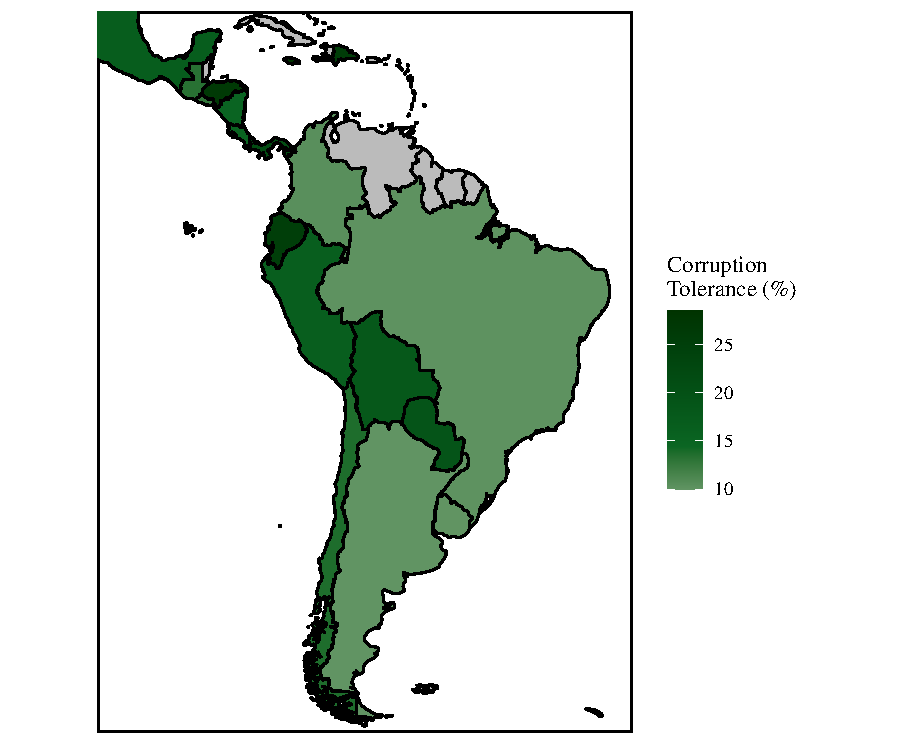
\includegraphics{images/ctol_map.pdf}
      \end{center}
      \textbf{Note:}
      A choropleth map showing corruption tolerance percentages across Latin America in 2019, where Ecuador places third in        the most corruption tolerant countries. Darker areas imply higher percentages of corruption tolerance. Figure                prepared by the author with data from the \textregistered AmericasBarometer 2018/19. 
    \end{minipage}
  }
\end{figure}

Corruption, if framed as any kind of inappropriate use of common power to benefit a select few at the expense of others \parencite{Warren.2004}, affects Ecuadorians extensively in their daily lives. According to \textcite{AlarconSalvador.2020}, up to 1.5 billion USD may be have been lost in 2019 due to corrupt practices in public contracting. During the decade-long Revolución Ciudadana regime, the local Anti-Corruption Comission estimates a 35 billion USD cost of corruption \parencite{RoaChejin.2020}. Ecuador has also seen increased COVID-19 vaccine inequality as top public officers inoculated non-priority subjects in their private circles \parencite{Taj.2021}, weakened public health services (\cite{Celi.2020}; \cite{Comercio.2021}; \cite{RoaChejin.2020}), policymakers charging fees for political positions (\cite{Espinosa.2021}; \cite{Gonzalez.2021}), lost Social Security funds \parencite{Pesantes.9152020}, among others. With the impairment of so many public services which Ecuadorians pay for and depend on, it would be expected that corrupt activities become publicly denounced and repudiated.

% Corruption Tolerance Time Series Graph

\begin{figure}[htbp]
\centering
\fbox{
\begin{minipage}{\textwidth}
\caption{Percent of Ecuadorians who justify corruption, by year}
\label{fig:ctoly}
\begin{knitrout}
\definecolor{shadecolor}{rgb}{0.969, 0.969, 0.969}\color{fgcolor}

{\centering 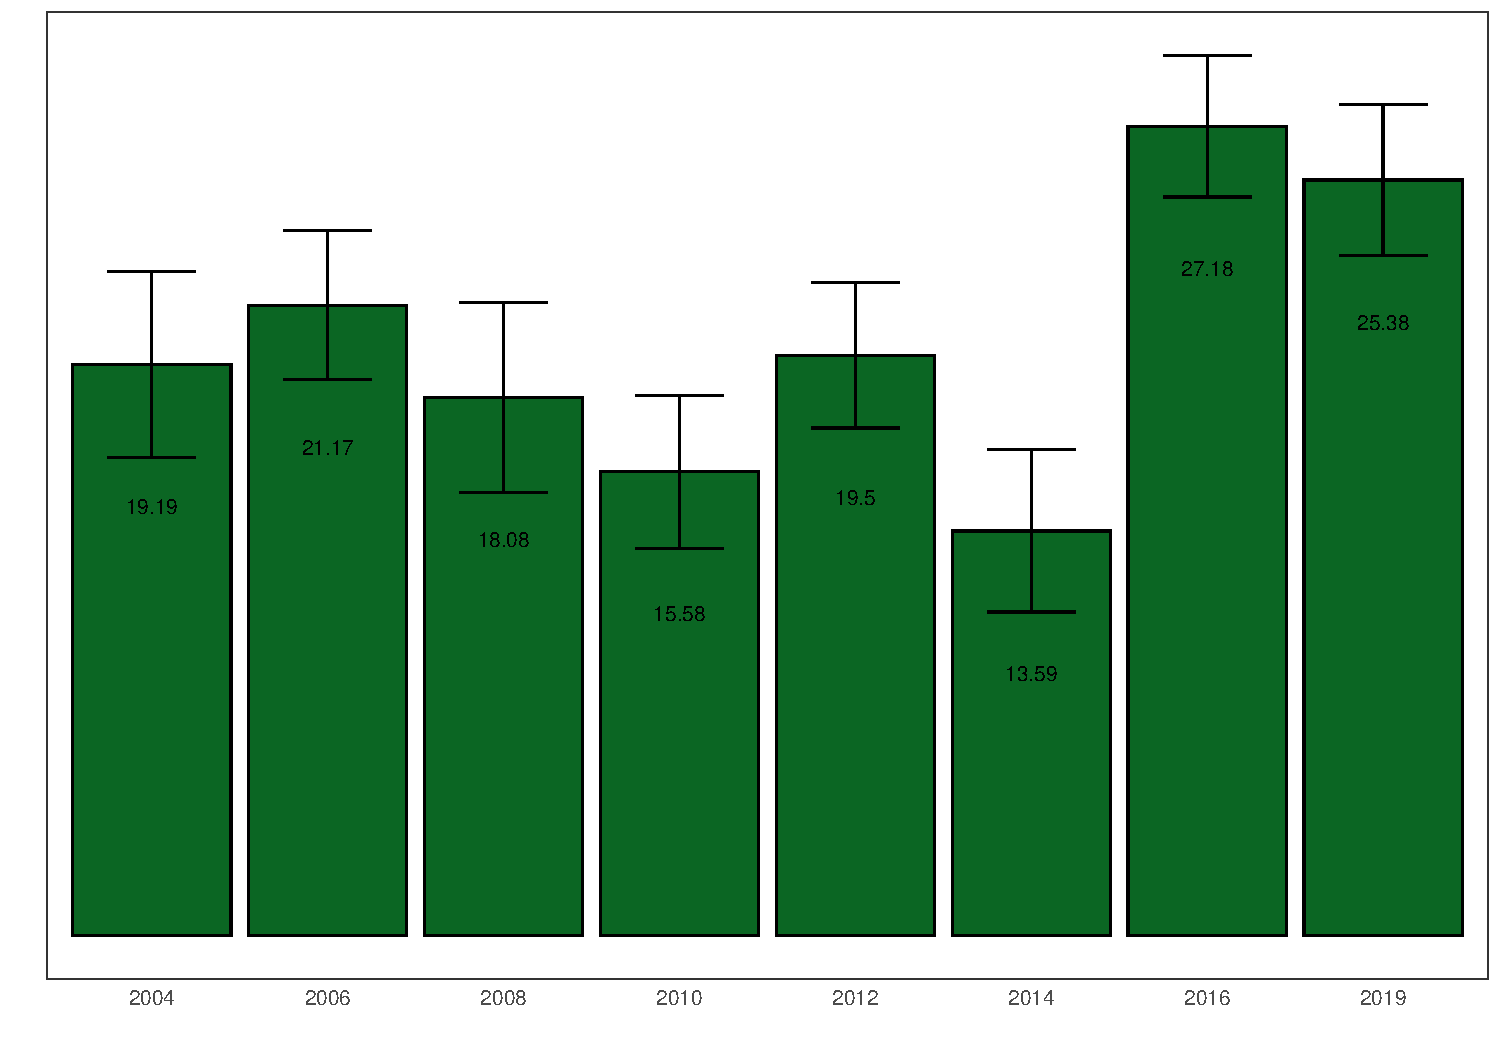
\includegraphics[width=\maxwidth]{figure/ctol_graph-1} 

}


\end{knitrout}
\textbf{Note:} The evolution of corruption tolerance for Ecuador. The largest increase is seen from 2014 to 2016. Error bars show 95\% confidence intervals, considering survey design effects. Figure prepared by the author, with the open-access AB data.
\end{minipage}}
\end{figure}

The largest increase in corruption tolerance was seen from 2014 to 2016, as it can be seen in Figure \ref{fig:ctoly}, where it increased from a historical low of 13.59 to a high of 27.18\%. This period coincides with two key events in the country. First, the popularity of a left-leaning and apparently omnipotent regime sharply dropped among accusations of corruption and poor management of the economy \parencite{Quillupangui.2016}. Second, a considerable economic recession hit the country which was mostly attributable to a commodity price collapse \parencite{Weisbrot.2017}. 

This study aims to explain the jump in corruption tolerance using survey data from the America's Barometer. The empirical analysis provides evidence that changes to the public's support of the political regime as well as a deteriorating economic environment came into play to increase corruption tolerance. The individual-level and across-time approach is a novelty in corruption literature and could be a better empirical approach to these kinds of research questions, as omitted-variable biases can be better controlled compared to cross-country approaches \parencite{Bergh.2017}. 

The mentioned events may have interacted with each other to cause political and economic turmoil as presidential elections approached in 2017 and many questioned the regime for the first time. Apart from the deterioration of the economy, the rule of President Rafael Correa saw its approval rating drop -15 percentage points according to the AB. These are significant changes in public opinion, so it is sensible to look at these as potential drivers for the increase in corruption tolerance. It should also be noted that historically, Ecuadorian citizens have tended to recognize corruption as an inevitable consequence of any political process, seemingly imagining a trade-off between corruption and public goods \parencite{Adoum.2000}. This account was confirmed by another public opinion in 2018, which estimates that 44\% of Ecuadorians justify corruption if it is done in exchange of goods and services provided by the public sector \parencite{Loaiza.2019}. Additionally, \textcite{Hurtado.2007} and \textcite{Adoum.2000} recognize multiple behavioral patterns in Ecuadorian citizens which lead to attitudes of resignation to the mechanisms of corruption, which may normalize corruption and thus create environments that foster its growth. 

Changes to the attitudes toward corruption can be as important to understand as the consequences or causes of actual corruption. First, a higher degree of corruption tolerance will eventually lead to larger corruption environments \parencite{Campbell.2014}. Social sanctions or rewards can significantly affect outcomes according to \textcite{Akerlof.1980}, even if these lead to smaller economic payoffs. Higher tolerance to corrupt acts, such as bribing, will mean that the social sanction of engaging in them is smaller, hence making the total payoff of the corrupt action higher, since a positive economic payoff to the corrupt individual is implied \parencite{Shleifer.1993}. However, corruption almost always entails that the economic payoff to the corrupt individual is done at the expense of the majority \parencite{Warren.2004}, thus affecting outcomes across all society, notably economic development and political stability \parencite{Singer.2016}. It thus becomes of prime importance to learn what drives corruption tolerance to be able to foster better policy-making and citizen attitudes which drive citizens away from enacting in and justifying corrupt actions.




% Literature Review Child Document


% Literature Review Rnw File


\section{Literature Review}

The literature has often focused on the specific causes, consequences and the incidence of corruption, as well as the public's perception of it. While it is mostly agreed that corruption is pervasive for societies both economically and politically, and mass media constantly denounces acts of corruption, many people justify these acts anyway. Lesser attention has been given to the corruption tolerance phenomenon in the literature. Before studying how this phenomenon works it is adequate to place corruption in a basic framework which will inform the way that people behave around it. 

A simple model of the motivations for corruption can be considered. On one hand, there is the potential (individual) payoff for engaging in corrupt acts, which are often of economic nature. \textcite{Shleifer.1993} model bribes with a microeconomic model, where the public official trades public goods in exchange for bribes. Private agents then pay them to receive the good and the consumer surplus that any transaction brings. This might be understood as an individual economic incentive to engage in corrupt acts: paying the bribe allows the use of a desirable public good, or allows for quicker access to it. Thus, economic convenience could be an important determinant of how people behave around corruption: people may tolerate dishonesty if it means a positive economic payoff. 

On the other hand, there might be also moral considerations to the decision of tolerating or engaging corruption. While the economic payoff of paying or receiving a bribe may be positive, the moral connotation of the act may bring shame or rejection from society. Avoiding a bad image may very well become an important determinant of the decision of engaging in a corrupt act. Nevertheless, in environments where corruption is tolerated the negative social payoff of bribing might be smaller, which increases incentives for being corrupt. The importance of social payoffs for economic transactions cannot be neglected, as according to \textcite{Akerlof.1980} these might change economic outcomes in a significant way, deviating from the equilibria derived from the assumptions of rational self-interested behavior. It then becomes key to understanding how the social payoffs of corrupt acts are determined, as it could be assumed that most of the time the economic payoff of bribes is positive for the corrupt individual. 

\textcite{Ariely.2019} discuss experimental findings which show that individuals that pay a bribe or are requested to pay one are more likely to behave dishonestly in subsequent ethical dilemmas. Further experimental evidence from \textcite{Gino.2009} also shows that subjects with more exposure to dishonest behaviors are more likely to engage in it. An empirical study of corrupt organizations by \textcite{Campbell.2014} shows that corrupt acts create an organizational culture which fosters the incidence of corruption among its members. The corrupt culture may change the behavior of otherwise honest individuals through social pressure, notably when philosophies where the ends justify the means are considered. These findings suggest that social norms and outer circumstances shape the way in which corruption is interpreted by the members of organizations. In this paper, the organizational culture may enclose the complete political apparatus of a country but also the more diffuse organizations that political affiliations represent. 

\textcite{Ashforth.2003} develop a theoretical model to explain how corruption is normalized or tolerated in an organization. They argue that after an initial exposure to corruption brought by several environmental factors (relaxed legal enforcement, permissive ethical climate, necessity, etc.), the corrupt decision starts being used in the future by organization members. Corrupt behavior then becomes part of the organizational culture or becomes \textit{institutionalized}, as the corrupt acts start to be considered as routine for the organization.  

Leadership in the organization is crucial for the initial stages of the institutionalization process. Leaders need not engage in corrupt acts themselves to foster their normalization, they can simply facilitate or ignore the initial corrupt acts to have subordinates start normalizing corruption. Moreover, strong rewards or punishments for engaging or not engaging in corrupt acts, as well as a strong emphasis on results also may lead to the institutionalizaton of corruption. Subordinates do not second-guess their superiors' decisions as a result of the habit of obedience, which is more prevalent in highly hierarchical organizations. The authors also note that the psychological process of obedience also comes with a sense of helplessness and resignation, where the subordinate becomes detached from the moral dilemma by thinking that they are only following orders. 

Along with the institutionalization of corrupt acts, two other mechanisms are involved in the normalization of corruption. These three mechanisms reinforce each other so that individuals in corrupt organizations do not believe they are corrupt when engaging in dishonest acts as bribes. The \textit{rationalization} mechanism of corruption in an organization is especially important for these attitudes. The authors argue that corrupt individuals rationalize corruption in a way that they \enquote{avoid the adverse effects of an undesirable social identity} \parencite[p.13]{Ashforth.2003}. Rationalization is based on the behavioral premise that the members of an organization may try to resolve the ambiguity that surrounds action in a way that it serves their own interests. 

There are several ways through which the mechanism of rationalization appears. One of them is the \textit{denial of responsibility}, in which corrupt individuals convince themselves that they have no other choice than to engage in corrupt acts due to external circumstances. The authors also consider the case when individuals see their own corruption as a form of revenge against unfair or corrupt acts done to them. A related type of rationalization is when corrupt acts are justified because the actors perceive those that denounce corruption as illegitimate or hypocritical authorities, charged with motives other than the well-being of the organization.

The final normalization mechanism is the \textit{socialization} of corruption. This mechanism is concerned with \enquote{teaching} corrupt practices to organization's newcomers. Newcomers to a corrupt organization are initially induced to change their attitudes towards corrupt beliefs, then being peer-pressured to escalate these practices. Since newcomers strive to be accepted, they end up adopting these dishonest behaviors as their own, while they also rationalize it to avoid the social costs of being dishonest. Then the newcomers become \enquote{experts} in these corrupt practices and are the ones that exert peer pressure on future members.

\textcite{Adoum.2000} describes how Ecuadorian citizens tend to surrender to an inefficient political system and to dishonesty: they recognize the system as corrupt but still do not fully condemn it. From this, Adoum suggests that the feeling of impotence within a corrupt system makes average citizens feel that the law is illegitimate and thus break it whenever it suits them without any kind of remorse. This is an interesting application of \textcite{Ashforth.2003} who suggest that dishonest behavior is rationalized by rejecting the legitimacy of authorities or view corruption as revenge for unfair acts. Adoum also confirms the idea that citizens who engage in dishonest behavior do not perceive themselves as corrupt by pointing to how detached the average Ecuadorian feels from the political process. Likely, this makes it easier to engage in \enquote{petty} dishonest acts.

\textcite{Hurtado.2007} claims that the Ecuadorian society has been historically prone to dishonest behaviors as a result of low economic development, feudalism in early Ecuadorian settlements, the effect of Spanish hierarchical culture, racism, extreme catholicism, inmoderate collectivism, among others. Hurtado holds that for a long time the Ecuadorian society has functioned with unfair and dishonest social and economic mechanisms, like political clientelism and nepotism for job hirings, disrespect to property rights, non-compliance with social and legal contracts, etc. It is suggested that these practices have hindered social and economic mobility, especially for historically marginalized ethnic groups. This makes dishonest behaviors even more widespread: a self-fulfilling prophecy of dishonest and pervasive behavior. 

\textcite{Loaiza.2019} provides a recent account of some of the mentioned author's claims. \textcite{Loaiza.2019} cites the Latinobarómetro survey, which finds that 44\% of Ecuadorians \enquote{are willing to accept crimes against the public administration - in other words, corruption- in exchange for basic services, public buildings or roads} (Loaiza, 2019, para. 5). This estimate places Ecuador as the sixth most tolerant country to corruption in Latin America. The survey confirms the findings of the AB, as it concurs in how Ecuadorians do not consider corruption as the most important problem and how it is perceived to be very widespread. The author also suggests a self-interest theory to justifying corruption, as about 11\% believe that it is better to be an accomplice of corruption than to denounce it. 

The corruption tolerance variable of the AmericasBarometer has been studied for both the Ecuadorian case as well as in the whole Latin-American region. \textcite{Singer.2016} find that for every country in Latin America in 2014, at least 60\% of the respondents perceive their governments to be corrupt but a much smaller proportion considers corruption to be the most important problem in their countries. The authors also find that the people most likely to justify corruption are those who have actually paid a bribe in the past. Other statistically significant determinants of corruption tolerance in 2014 are age, where younger respondents justify it more as well as living in an urban setting, wealth and crime victimization. They also find that people who have paid bribes and also receive government assistance are more prone to justify corruption. This could serve as evidence for the previously mentioned claim that Ecuadorians trade-off public goods with corruption.

\textcite{Lupu.2017} further shows that corruption tolerance has been growing consistently in the region and that the average Latin American country has about a fifth of its population believing that corruption is justified. Between 2014 and 2016, corruption tolerance grew from 17.4\% to 20.5\% in the region. It is found that wealthier, older citizens as well as those who have been exposed to corruption are more prone to justify it. However, the number of children in the household was now positively related with corruption tolerance as well as the level of perceived corruption, while the government assistance indicator was no longer a significant predictor. \textcite{Lupu.2017} also gives the worrying conclusion that corruption may have become a \enquote{a self-fulfilling prophecy: as more and more citizens perceive that corruption is more widespread, they also become more likely to condone it}(p. 67). 

Finally, regarding Ecuadorians' corruption tolerance behaviors, \textcite{Moscoso.2018} find that corruption is perceived to be very widespread in the country yet it is not regarded as an important. It is also noted that for 2016, Ecuador became one of the countries which was the most tolerant of corruption, only below Haiti and the Dominican Republic. \textcite{Montalvo.2019} finds that the general Latin American trend for younger people to justify corruption more is also found in Ecuador. For the same round, \textcite{Moscoso.2020} find that besides age, interest in politics is a statistically significant predictor as well as exposure to corruption\footnote{The original wording by the authors in the LAPOP AB reports is \textit{corruption victimization}. Here, this variable is referred to as \textit{corruption exposure}, to account for the possibility that the respondent can be either a victim of corruption by being forced to pay a bribe or the initial corrupt agent who offers to pay one.}, as found by \textcite{Lupu.2017}. According to these authors, the empirical evidence may very well support the fact that corruption has become a known inconvenience for daily Ecuadorian life rather than an unacceptable threat to the system, and that it is endemic to the political and social environments. 




% Methodology Child Document


% Methodology .Rnw File


\section{Methodology}
\label{sec:methodology} % Label the section to cross-reference later.
\subsection{Data}

To study corruption at the individual level, the AmericasBarometer (AB) survey from the Latin American Public Opinion Project (LAPOP) is used. This survey was administered in Ecuador in a face-to-face interview format from 2004 to 2019 at mostly two year intervals. It asks about several matters, including democracy, corruption, political processes, economic considerations, among others. Some of the data used in this paper comes from the copyrighted \textregistered AmericasBarometer survey, financed by Universidad San Francisco de Quito. Most of the data comes from the open-access AmericasBarometer databases available in the LAPOP \href{https://www.vanderbilt.edu/lapop/data-access.php}{website}. Table \ref{tab:descrip} presents descriptive statistics computed for all variables used in the study.

The empirical models estimated in this study will use the survey data from the 2014 and 2016 rounds in Ecuador, with $n_{2014}=1489$ and $n_{2016}= 1545$. The survey is based on a multi-stage national probability design, with a stratification by region (Costa, Sierra, Amazonía). Each of these major strata were substratified by size of municipality and urban/rural areas \parencite{LAPOP.2017}. The errors for each of these surveys, incorporating design effects, are $\pm 2.5\%$ and $\pm 1.9\%$, respectively (\cite{LAPOP.2014}; \cite{LAPOP.2017}). Both of the surveys are self-weighted, however, 95\% confidence intervals for the descriptive statistics which are adjusted for design-effects are presented when relevant. 

% Here I will create a descriptive table including averages (and proportions) by year.
% This table is a bit difficult to construct because of its survey-weighted statistics and the rather complex structure, which is why I created it using Excel, exporting the results from calculations 
\begin{table}[htbp!]
\onehalfspacing
\begin{center}
\caption{Descriptive statistics for all variables used in the empirical models}
\label{tab:descrip}
\begin{tabular}{llcccc}
\toprule
\multicolumn{1}{c}{\multirow{2}{*}{Variable}} & \multirow{2}{*}{\begin{tabular}[c]{@{}l@{}} Question code \end{tabular}} & \multicolumn{2}{c}{2014}  & \multicolumn{2}{c}{2016}  \\ 
\cmidrule(l{3pt}r{3pt}){3-4} \cmidrule(l{3pt}r{3pt}){5-6}
\multicolumn{1}{c}{}                          &                                                                                         & Est. & SE & Est. & SE \\ \midrule
Corruption tolerance                          & EXC18                                                                                   & 13.59    & 1.39           & 27.18    & 1.21           \\
Unemployment                                  & OCUP4A                                                                                  & 10.06    & 1.04           & 22.89    & 1.2            \\
Confidence in the President                   & B21A                                                                                    & 69.01    & 1.77           & 49.64    & 1.49           \\
Approval of the President                     & M1                                                                                      & 70.26    & 1.57           & 55.41    & 1.43           \\
Economic situation (Worse)                            & IDIO2                                                                                   & 22.93    & 1.26           & 51.76    & 1.45           \\
No political wing                             & L1                                                                                      & 21.49    & 2.11           & 8.67     & 0.74           \\
Center                                        & L1                                                                                      & 42.58    & 1.92           & 45.7     & 1.49           \\
Left                                          & L1                                                                                      & 22.23    & 1.25           & 22.46    & 1.24           \\
Right                                         & L1                                                                                      & 13.7     & 1.16           & 23.17    & 1.15           \\
Women                                         & Q1                                                                                      & 50.37    & 0.34           & 50.29    & 0.3            \\
Age                                           & Q2                                                                                      & 39.41    & 0.17           & 38.64    & 0.22           \\
Years of education                            & ED                                                                                      & 10.67    & 0.15           & 11.43    & 0.14           \\
Urban                                         & UR                                                                                      & 65.21    & 4.11           & 66.41    & 4.07           \\
External political efficacy                   & EFF1                                                                                    & 35.31    & 1.69           & 41.93    & 1.33           \\
Internal political efficacy                   & EFF2                                                                                    & 38.55    & 1.58           & 41.49    & 1.34           \\
Participated in a protest                     & PROT3                                                                                   & 6.82     & 0.89           & 4.67     & 0.55           \\
Interest in politics & POL1 & 33.45 & 1.63 & 32.29 & 1.35 \\
Perceives corruption                          & EXC7, EXC7NEW                                                                           & 70.29    & 1.74           & 83.49    & 0.97           \\
Exposed to corruption                         & EXC 2,6,11,13,14,15,16                                                                  & 26.97    & 2.01           & 27.69    & 1.23           \\ 
\bottomrule
\end{tabular}
\end{center}
\doublespacing
\textbf{Note:} Descriptive statistics table with estimates (Est.) and robust standard errors (SE), where age, years of education and the external and internal political efficacies are arithmetic means. All other variables are percentages, calculated for 2014 and 2016 as seen in \hyperref[app:first]{Appendix A}. Standard errors adjusted for design effects. Question codes come from the AB survey questionnaires. Data from the open-access AB databases.
\end{table}

\subsection{Empirical Models}

The empirical analysis is concerned with the answers to the \emph{EXC18} question in the AB interviews: 
\enquote{Do you think given the way things are, sometimes paying a bribe is justified?} \parencite[p.96]{Moscoso.2018}, asked originally in Spanish. The question has been asked in all survey rounds in Ecuador and is the last one after a set of questions regarding corruption exposure and perception. The corruption tolerance variable ($ctol$) takes the value of 1 when the respondent answers \enquote{Yes}, 0 when they answer \enquote{No} and for any other responses the observation is dropped from the models. All models have $ctol$ as their dependent variable. Responses to other questions of the AB in these periods are used as regressors, and their encodings are explained in detail in \href{app:first}{Appendix A}.

In order to identify the changes in public behavior which led to the increase in corruption tolerance, observations from both surveys are pooled and the following general model is estimated: 
\begin{equation}
\label{eqn:genmod}
P(ctol = 1 | \textbf{\textit{X}} \hspace{0.04cm}) = G (\textbf{\textit{X}} \theta ) = G \left[ \beta_0 + \delta_0 y_{16} + \textbf{\textit{R}}\beta + \delta_1 (y_{16} \cdot x^*) \right]
\end{equation}
where $\textbf{\textit{R}}$ is a vector of important explanatory variables for $ctol$ and $x^*$ is a key regressor whose change across time may have significantly influenced the rise of $ctol$ between 2014 and 2016. This key regressor is interacted with a year dummy $y_{16}$ which equals unity for 2016 observations. The complete regressors' vector $\textbf{\textit{X}}$ includes all variables in $\textbf{\textit{R}}$ and the interaction term. The vector $\theta$ includes the coefficients vector $\beta$ as well as the intercepts $\beta_0$ and $\delta_0$ and the $\delta_1$ coefficient. $G$ is the link function, which can be unity for a linear probability model, or be equal to the logit and probit functions.

The partial effect of the key regressor $x^*$ on $P(ctol =1| \textbf{\textit{X}})$ will be:
\begin{equation}
\label{eqn:keype}
\dfrac{\partial P(ctol = 1 | \textbf{\textit{X}} \hspace{0.04cm})}{\partial x^*} = \dfrac{\partial G}{\partial \theta} \cdot 
\dfrac{\partial \theta}{\partial x^*} = G'(\theta) \cdot (\beta_{x^*}+ \delta_1 y_{16})
\end{equation}
Therefore, the coefficient of interest in this study is $\hat{\delta}_1$, which would measure the ceteris paribus effect of a change in the key regressor $x^*$ from 2014 to 2016 in the dependent variable $ctol$. If there has been a change in 2016 in the $x^*$ which influences corruption tolerance, $\hat{\delta_1}$ should be statistically significant. 

A $\hat{\delta}_1$ coefficient which is not statistically different from zero would mean that individuals with and without this key characteristic are equally likely to justify corruption across time. Additionally, if $\hat{\beta}_{x^*}$ and $\hat{\delta}_1$ have different signs but similar magnitudes, the \enquote{net} effect might approach zero. 

To better understand these potential cases, the following single cross-section models are also estimated:
\begin{equation}
\label{eqn:crosssecmodel}
P(ctol = 1 | \textbf{\textit{R}}_y \hspace{0.04cm}) = G (\textbf{\textit{R}}_y \beta_y) = G[\beta_{y,0} + \beta_{y,x^{*}} + \beta_y \textbf{\textit{X}} ]
\end{equation}
for either $y=2014$ or $y = 2016$. The vector $\textbf{\textit{R}}_y$ incorporates important explanatory variables for period $y$, including the key variable $x^*$ for the period in question. The magnitudes of the $\hat{\beta}_{y, x^*}$ should be similar between the two periods when $\hat{\delta}_1$ is not statistically different from zero in the pooled cross-sections model of Equation \ref{eqn:genmod}. Also, $\hat{\beta}_{y,x^*}$ for 2016 should not be statistically different from zero if $\hat{\beta}_{y,x^*}$ cancel each other out in the pooled cross-sections model. 

Average partial effects tables are shown for all models estimated in this paper. The \hyperref[sec:findings]{Results} section includes only the logit estimations of each empirical model. LPM and probit estimations of the models are included in the appendices, along with the average partial effects for the probit models.

The individual level approach that all of these models use might be more empirically accurate than a cross-national approach which pools national averages across countries. As mentioned before, this approach is less likely to omit important variables \parencite{Bergh.2017}. Also, this approach might reflect general perceptions and incidence of corruption more accurately. This is because country-level indicators are based on opinions from experts whereas the AB proportions capture the opinion from all citizens \parencite{Morris.2008}. However, results found using this approach are likely less applicable to countries other than the one studied. Besides, since there is no tracking individuals across time using the AB survey panel-data methods cannot be implemented. 

\subsection{Incorporating design effects}
All models use survey-weighting to adjust for the complex sample design effects, as suggested by \textcite{Castorena.2021} for the use of AB survey data on research projects. In the Ecuadorian case, surveys from 2014 and 2016 are self-weighted, so the survey-weighting does not affect coefficient magnitudes or average partial effects. However, the design effects do change standard errors for all coefficients. Survey-weighted standard errors are presented in this paper for both model coefficients and average partial effects. 


% Results 1 Child Document


% Results I .Rnw File


\section{Results}
\label{sec:findings}
\subsection{Potential drivers of the increase in corruption tolerance}
As pointed out previously, the corruption tolerance increase happened at the same time as other key events. First, AB indicators denote a political crisis, as support for President Rafael Correa's regime took a sharp hit. Second, a recession hit Ecuador due to a commodity price collapse, an earthquake and other circumstances. Below, Figure \ref{fig:ecua_pol} shows several public opinion indicators and Figure \ref{fig:ecua_ec} displays economic conditions, both observed and perceived from 2014 to 2019. 

% Create the data to be used for the political opinion variables:

% Now do the graph
\begin{figure}[htbp]
\centering
\fbox{
\begin{minipage}{\textwidth}
\caption{Ecuadorian public opinion indicators, 2004-2019}
\label{fig:ecua_pol}
\begin{knitrout}
\definecolor{shadecolor}{rgb}{0.969, 0.969, 0.969}\color{fgcolor}

{\centering 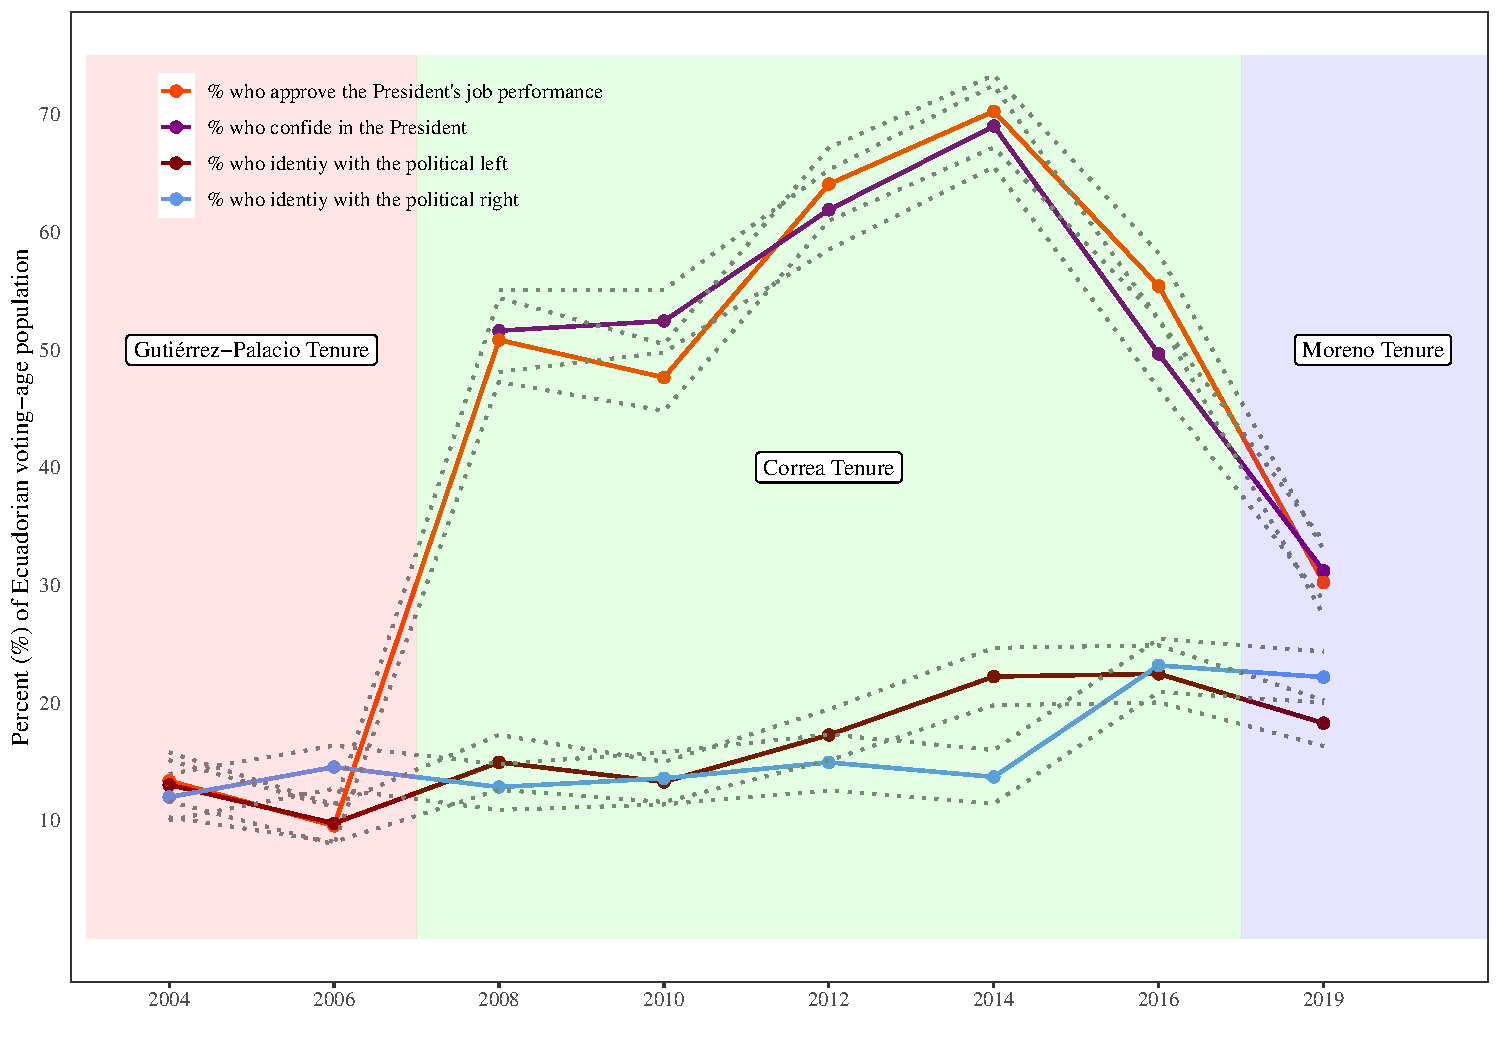
\includegraphics[width=\maxwidth]{figure/political_graph-1} 

}


\end{knitrout}
\textbf{Note:} The graph shows time series for political public opinion questions asked in the AB. Percentages are estimated as explained in \hyperref[app:first]{Appendix A} and error bars show 95\% confidence intervals considering design effects. Figure prepared by the author. \end{minipage}
}
\end{figure}

The AB data shows that indeed the President reached an all-time high popularity in 2014 and then a severe drop in 2016. This is seen through the percent of people who approve the President's job performance and the percent who report confidence in him. Another notable change in the political landscape is the way that voting-age population politically identified. There was a strong increase of the people who identified as the \enquote{right}, while those who identified with the \enquote{left} did not see significant changes.

Regarding the economic recession, \textcite{Orozco.2015} holds that although the commodity price collapse in 2008 was greater, there was little reduction in economic activity as the country had greater possibilities of international financing and savings left over from past oil funds, which were used to keep government expenditure high. In 2016, as savings eroded and government debt had grown bigger, the economy stagnated significantly for the first time in the Correa administration. Combined with the lack of competitiveness in exports due to US dollar appreciations and the poor public finance administration \parencite{Hurtado.2018}, the country fell into a deep economic recession. While the official GDP figures may show only a small reduction in GDP growth, \textcite{Hurtado.2018} holds that these figures are overestimated.

% Here I create my graph, but I need to load some libraries first and create the data needed for my graphs.

% Now I do the graph:
\begin{figure}[htbp]
\begin{center}
\fbox{
\begin{minipage}{\textwidth}
\caption{Ecuadorian economic conditions 2004-2019}
\label{fig:ecua_ec}
\begin{knitrout}
\definecolor{shadecolor}{rgb}{0.969, 0.969, 0.969}\color{fgcolor}

{\centering 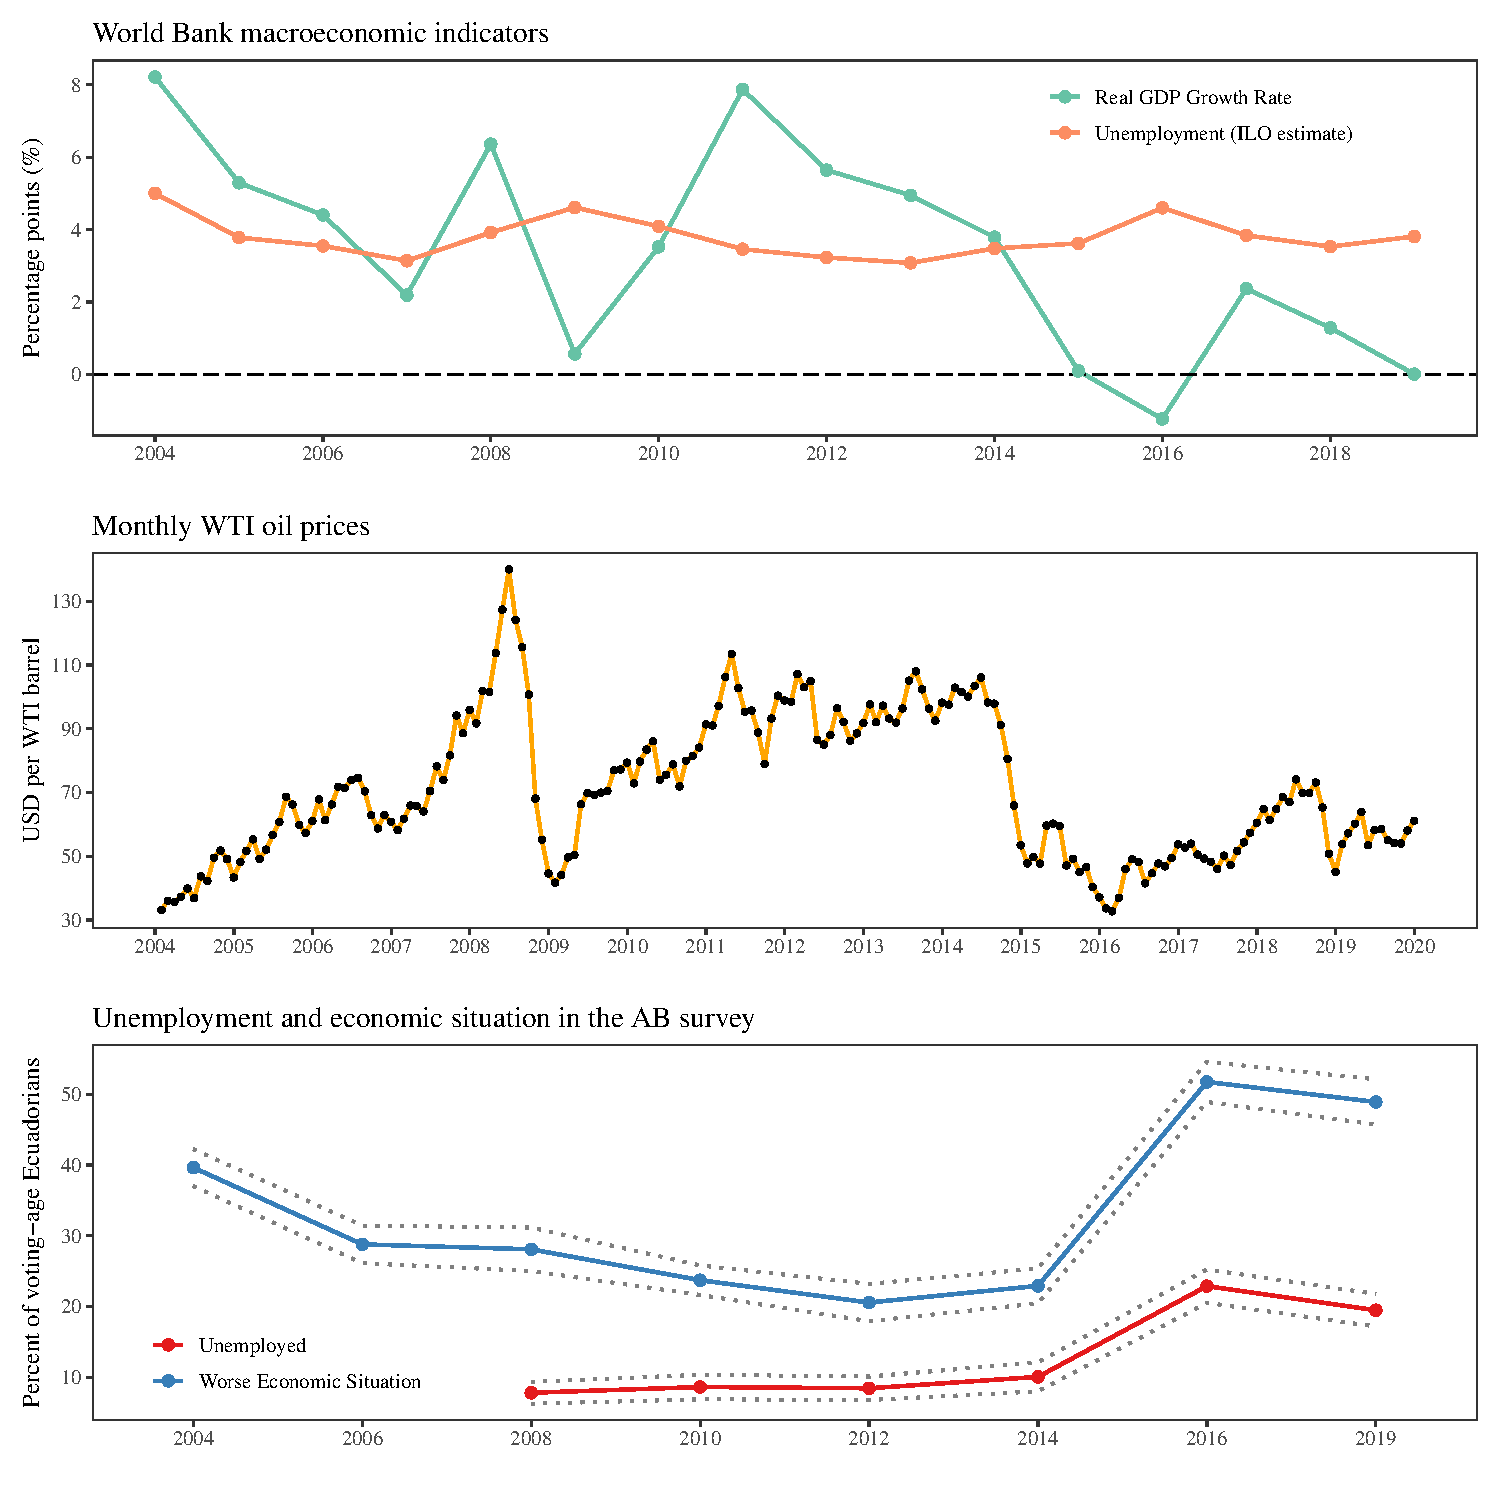
\includegraphics[width=\maxwidth]{figure/econ_graph-1} 

}


\end{knitrout}
\textbf{Note:} Time series line graphs showing key economic indicators for the country between 2004 and 2019. Real GDP growth and unemployment rates extracted from the World Bank's World Development Indicators. WTI oil barrel prices extracted from FRED. The rest are estimates computed with the open-access AB databases, which include 95\% confidence intervals adjusted for design effects. See \hyperref[app:first]{Appendix A} for details on calculations. Figure prepared by the author. 
\end{minipage}}
\end{center}
\end{figure}

Figure \ref{fig:ecua_pol} shows several indicators of public opinion in the country. The AB data shows that indeed the President reached an all-time high popularity in 2014 and then a severe drop in 2016. This is seen through the percent of people who approve the President's job performance and the percent who report confidence in him. Another notable change in the political landscape of this period is the way that voting-age population identified politically. There was a notable increase of the people who identified as the \enquote{right} of the political wings, while those who identified with the \enquote{left} did not see significant changes.




% Results 2 Child Document


% Results II .Rnw File

\subsection{Baseline regressions}
\label{subsec:fin2}

Based on the previous subsection's findings, some potential key determinants for corruption tolerance are considered. Two economic variables at the individual level significantly changed during this period: the percent of people who report a worse economic situation as well as the indicator of unemployment. These follow macroeconomic indicators for the Ecuadorian economy too, as can be seen in Figure \ref{fig:ecua_ec}. Variables which proxy attitudes in the political landscape also have significantly changed: the percentage of people who confide in the President, the percentage who approve the President's job and also the percentage of people who identify with the political right wing.

Simple empirical models are estimated to study the relationship of these key changes with corruption tolerance, which follow the equation below:
\begin{equation}
\label{eqn:simplemod}
P(ctol = 1 | \textbf{\textit{X}} \hspace{0.04cm}) = G \left[ \beta_0 + \delta_0 y_{16} + \beta_1 x^* + \delta_1 (y_{16} \cdot x^*) + u\right]
\end{equation}
where $x^*$ is the key regressor, which can either be: 
\begin{itemize}
  \item A dummy variable set to unity for respondents who answered that their economic situation is worse (Model 1)
  \item A dummy variable set to unity for respondents who report being unemployed (Model 2)
  \item A discrete variable with numbers 1-7, where higher numbers imply a higher degree of confidence in the President (Model 3)
  \item A discrete variable with numbers 1-5, with higher numbers implying a higher rating of the President's job performance (Model 4)
  \item A discrete variable with numbers from 1-10 where 1 is the extreme left and 10 is the extreme right (Model 5)
\end{itemize}
% Now I'm going to run the first models, and I'll do so by sourcing a script.


% Now, I'll make the table with modelsummary from the sourced stuff. 
\begin{table}[htbp]
\caption{Logit coefficients for baseline models}
\label{tab:simplemodel}

\begin{tabular}[t]{lccccc}
\toprule
  & Model 1 & Model 2 & Model 3 & Model 4 & Model 5\\
\midrule
Constant & \num{-1.894}*** & \num{-1.989}*** & \num{-0.455}** & \num{0.553} & \num{-1.527}***\\
 & (\num{0.127}) & (\num{0.110}) & (\num{0.208}) & (\num{0.362}) & (\num{0.196})\\
2016 Dummy & \num{0.848}*** & \num{1.001}*** & \num{-0.188} & \num{-1.251}*** & \num{0.278}\\
 & (\num{0.158}) & (\num{0.132}) & (\num{0.238}) & (\num{0.415}) & (\num{0.234})\\
Worse Economic Situation & \num{0.131} &  &  &  & \\
 & (\num{0.169}) &  &  &  & \\
Unemployment &  & \num{1.015}*** &  &  & \\
 &  & (\num{0.205}) &  &  & \\
Confidence in President &  &  & \num{-0.288}*** &  & \\
 &  &  & (\num{0.037}) &  & \\
Approval of Pres. Performance &  &  &  & \num{-0.648}*** & \\
 &  &  &  & (\num{0.096}) & \\
Political Wing &  &  &  &  & \num{-0.047}\\
 &  &  &  &  & (\num{0.038})\\
Econ. Situation Interaction & \num{-0.025} &  &  &  & \\
 & (\num{0.197}) &  &  &  & \\
Unemployment Interaction &  & \num{-1.005}*** &  &  & \\
 &  & (\num{0.256}) &  &  & \\
Pres. Confidence Interaction &  &  & \num{0.206}*** &  & \\
 &  &  & (\num{0.044}) &  & \\
Pres. Approval Interaction &  &  &  & \num{0.568}*** & \\
 &  &  &  & (\num{0.111}) & \\
Pol. Wing Interaction &  &  &  &  & \num{0.095}**\\
 &  &  &  &  & (\num{0.043})\\
\midrule
$N$ & \num{2948} & \num{2950} & \num{2944} & \num{2941} & \num{2535}\\
AIC & \num{2893.64} & \num{2889.04} & \num{2848.57} & \num{2844.82} & \num{2574.81}\\
BIC & \num{2926.37} & \num{2920.98} & \num{2881.80} & \num{2876.65} & \num{2606.10}\\
\bottomrule
\end{tabular}


\vspace{0.25cm}
\textbf{Note:} Logit coefficients of the baseline models as described by Equation \ref{eqn:simplemod}. Standard errors consider design effects of the AB complex survey design.\\
*$p$ < 0.1, **$p$< 0.05, ***$p$ < 0.01.
\end{table}

Table \ref{tab:simplemodel} presents the logit estimates of the model coefficients for Equation \ref{eqn:simplemod}. The coefficient for the year dummy shows the significance of the jump in corruption tolerance for year 2016. This significance is lost when considering interaction terms with confidence in the President. The year dummy actually has a negative sign when the approval of his job performance and the political score variable are considered. While unemployment does seem to have a significant effect in year 2014 and also in an interaction term, its inclusion does not eliminate the significance of the year dummy. The coefficients also suggest that a person who reports having a worse economic situation does not tolerate corruption more or less than those who report a same or equal economic situation. 

Model 1 suggests that a person who reports having a worse economic situation does not tolerate corruption differently than those who report a same or higher economic situation. Model 2 shows that respondents who were unemployed were more likely to justify corruption than those who were not unemployed (either employed or not in the labor force, see \hyperref[app:first]{Appendix A}). The interaction term in this model has a negative sign, which shows that the effect of unemployment in 2016 was less than the effect in 2014. While this relationship would not clearly explain the jump in corruption tolerance, it is an interesting finding which will be explored further. 

Models 3 and 4 display the same relationship: people who either trust or approve of the President in a higher degree also tolerate corruption less. A more zealous supporter of the regime will believe that bribes are not justified given the actual situation, however, this appears to change in 2016. The interaction term for both variables are significant and positive: in 2016 regime supporters started to justify corruption in a higher degree relative to 2014 levels. This could explain the jump in corruption tolerance since support for the President eroded in 2016, which meant that the number of non-supporters was higher; these respondents justified corruption more than supporters. Also, the supporters that remained started to justify bribes to a higher degree for this year. In Model 3, the significance of the year dummy is lost, while in Model 4 its sign is reversed.

The political identification of respondents is taken into account in Model 5. The coefficients show that a person who identifies closer to the political right does not justify corruption differently relative to people identifying closer to the political left. However, the interaction term shows that people answering higher values of this variable justified corruption more in 2016. Once again, the significance of the year dummy is lost when considering this variable. With a higher number of respondents identifying with the political right wing, who appear to justify corruption more, it would be understood how overall corruption tolerance increased. This estimate, however, is less statistically significant than the other three interaction terms in the other models. 

All of these results hold with the logit and linear probability models, which can be seen in Appendix \label{app:second}. Table \ref{tab:apebase} presents average partial effects for the model estimations in Table \ref{tab:simplemodel}. Table \ref{tab:apesimp} presents average partial effects for the five models of Table \ref{tab:simplemodel}. These figures show that an unemployed person is 5.9\% more likely to justify corruption. Additionally, a respondent who answered one number higher for an increased degree of confidence in the President was 2.4\% less likely to justify corruption. Finally, a person who rated the President's job performance one unit higher was 4.4\% less likely to justify corruption. All other partial effects are not significant. Similar magnitudes are obtained for the probit model average partial effects, as seen in Table \ref{tab:probitsimpape}. 

% Do the APE table
\begin{table}[htbp]
\caption{Average partial effects for logit models in Table \ref{tab:simplemodel}}
\label{tab:apesimp}

\begin{tabular}[t]{lccccc}
\toprule
  & Model 1 & Model 2 & Model 3 & Model 4 & Model 5\\
\midrule
2016 Dummy & \num{0.848}*** & \num{1.001}*** & \num{-0.188} & \num{-1.251}*** & \num{0.278}\\
 & (\num{0.158}) & (\num{0.132}) & (\num{0.238}) & (\num{0.415}) & (\num{0.234})\\
Unemployment &  & \num{1.015}*** &  &  & \\
 &  & (\num{0.205}) &  &  & \\
Approval of Pres. Performance &  &  &  & \num{-0.648}*** & \\
 &  &  &  & (\num{0.096}) & \\
Political Wing &  &  &  &  & \num{-0.047}\\
 &  &  &  &  & (\num{0.038})\\
\midrule
$N$ & \num{2948} & \num{2950} & \num{2944} & \num{2941} & \num{2535}\\
\bottomrule
\end{tabular}


\vspace{0.25cm}
\textbf{Note:} Average partial effects for the models estimated in Table \ref{tab:simplemodel}. Data from the open-access AB databases. Standard errors consider design effects of the AB complex survey design.\\
*$p$ < 0.1, **$p$< 0.05, ***$p$ < 0.01.
\end{table}

% I need to draw the graph which shows the visual differences between groups and their corruption tolerance

% I draw my data by sourcing the tabulations script.



% Now I do the data wrangling needed for this


% Now do the graph
\begin{figure}[htbp]
\caption{Graphical representations of corruption tolerance across key explanatory variables}
\label{fig:difgraph}
\fbox{
\begin{minipage}{\textwidth}
\begin{knitrout}
\definecolor{shadecolor}{rgb}{0.969, 0.969, 0.969}\color{fgcolor}

{\centering 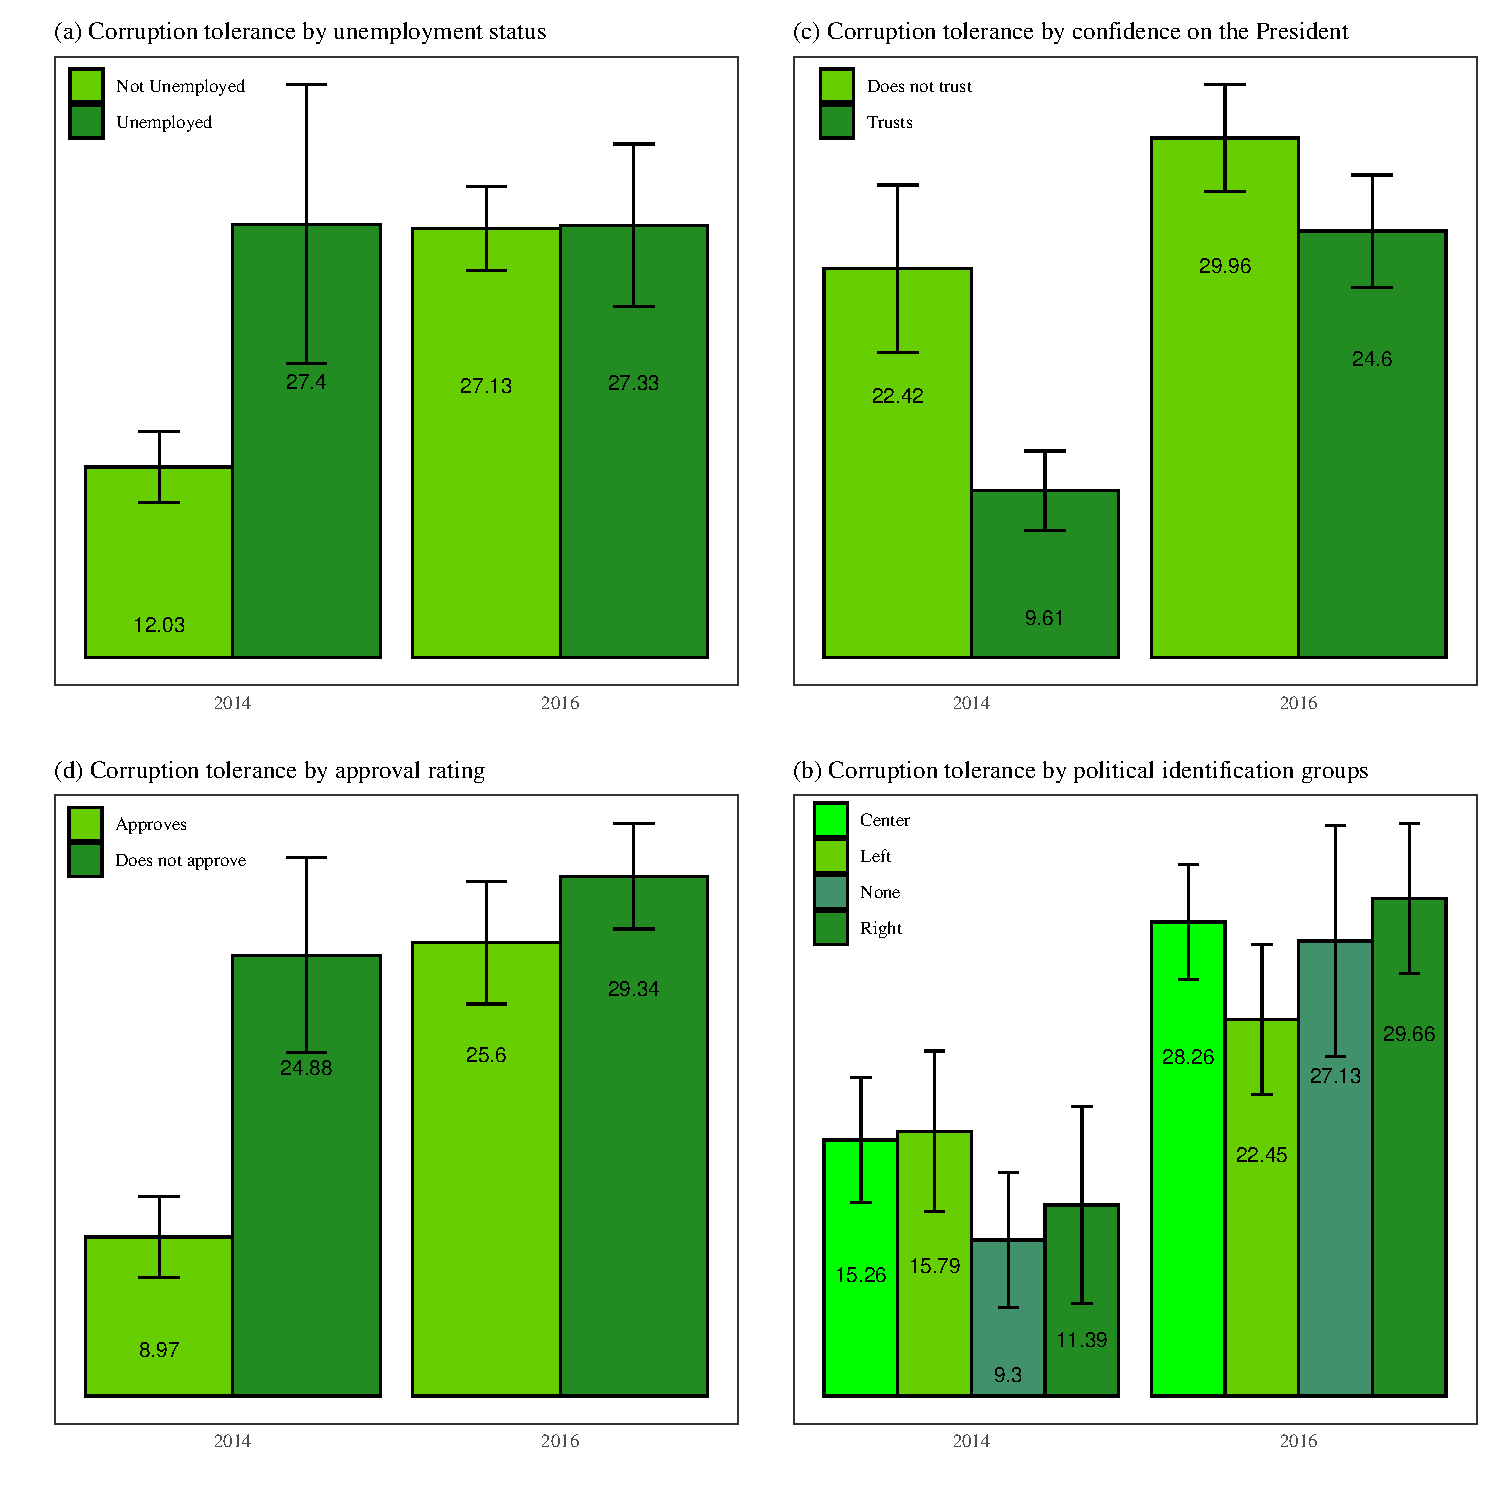
\includegraphics[width=\maxwidth]{figure/difgraph-1} 

}


\end{knitrout}
\textbf{Note:} Figures show the percent of respondents that justify corruption across the groups used as explanatory models in Table \ref{tab:simplemodel}. Data from the open-access databases of the AB. Error bars represent the 95\% confidence intervals considering design effects. Figure prepared by the author. 
\end{minipage}
}
\end{figure}

The findings of these models can be further explained by Figure \ref{fig:difgraph}. According to panel (a), in 2014, only 12.03\% of people who were not unemployed justified corruption, while in 2016 this figure increased to 27.03\%, very close to the percentage of unemployed people who justified it in 2016. The difference between time periods of these percentages is not statistically significant, which means that in 2016 the effect of unemployment in corruption tolerance approached zero. Thus, Figure \ref{fig:difgraph} along with Model 2 of Table \ref{tab:simplemodel} show that it was not the unemployed who started to justify corruption less, it was that the people who were not unemployed started to justify it more. Panels (b) and (c) of Figure \ref{fig:difgraph} show that the percentage of people who either confided in or approved the President and justified corruption increased significantly  between 2014 and 2016. This means that the negative effect of supporting the executive in 2016 was smaller than in 2014, as confirmed by the interaction term in Models 3 and 4 of Table \ref{tab:simplemodel}. In panel (d) of Figure \ref{fig:difgraph}, where four different political groups are considered: the left, right, center and those who did not answer the question. All four groups saw increases in the percent of group members who justify corruption. All increases in corruption tolerance are significant, except for those who identify with the left wing. This is consistent with the coefficient sign seen in Model 5 for the political score variable. 


% Results 3 Child Document


% Results III .Rnw File


\subsection{Ceteris paribus effects of unemployment, presidential approval and political identification on corruption tolerance}

Now the general model as described by Equation \ref{eqn:genmod} is estimated, where \textbf{R} is a vector of explanatory variables that the study of the literature on corruption tolerance and normalization suggests. The statistically significant relationships with interaction terms which were determined previously are kept as the key explanatory variables $x^*$, with the exception of the confidence in the president variable, as the presidential approval variable captures the same effects. Thus, three models are estimated, whose coefficients are shown in Table \ref{tab:complexmod}.

% Estimate the modified models, by sourcing that .R file



% Now create the table
\begin{table}[htbp]
\begin{center}
\caption{Logit coefficients for modified models}
\label{tab:complexmod}

\begin{tabular}[t]{lccc}
\toprule
  & Model 1 & Model 2 & Model 3\\
\midrule
Constant & \num{-0.674}* & \num{0.707} & \num{-0.351}\\
 & (\num{0.401}) & (\num{0.468}) & (\num{0.405})\\
2016 Dummy & \num{0.887}*** & \num{-1.217}** & \num{0.333}\\
 & (\num{0.145}) & (\num{0.477}) & (\num{0.252})\\
Woman & \num{0.124} & \num{0.136} & \num{0.127}\\
 & (\num{0.109}) & (\num{0.111}) & (\num{0.109})\\
Age & \num{-0.026}*** & \num{-0.026}*** & \num{-0.026}***\\
 & (\num{0.004}) & (\num{0.004}) & (\num{0.004})\\
Years of education & \num{-0.041}*** & \num{-0.038}** & \num{-0.039}**\\
 & (\num{0.015}) & (\num{0.015}) & (\num{0.015})\\
Lives in urban setting & \num{-0.020} & \num{0.013} & \num{0.009}\\
 & (\num{0.132}) & (\num{0.131}) & (\num{0.132})\\
External political efficacy & \num{-0.047} & \num{-0.041} & \num{-0.044}\\
 & (\num{0.032}) & (\num{0.032}) & (\num{0.032})\\
Internal political efficacy & \num{0.096}** & \num{0.093}** & \num{0.089}**\\
 & (\num{0.041}) & (\num{0.042}) & (\num{0.041})\\
Participation in a protest & \num{0.431}** & \num{0.450}** & \num{0.471}**\\
 & (\num{0.204}) & (\num{0.205}) & (\num{0.207})\\
Interest in politics & \num{-0.249}** & \num{-0.220}* & \num{-0.244}**\\
 & (\num{0.116}) & (\num{0.119}) & (\num{0.119})\\
Perceptions of corruption & \num{0.000} & \num{0.001} & \num{-0.033}\\
 & (\num{0.133}) & (\num{0.137}) & (\num{0.136})\\
Exposure to corruption & \num{0.985}*** & \num{1.003}*** & \num{1.008}***\\
 & (\num{0.115}) & (\num{0.114}) & (\num{0.115})\\
Unemployment & \num{0.956}*** & \num{0.296}** & \num{0.285}*\\
 & (\num{0.215}) & (\num{0.146}) & (\num{0.145})\\
Approval of Pres. Performance & \num{-0.132}** & \num{-0.510}*** & \num{-0.128}**\\
 & (\num{0.063}) & (\num{0.102}) & (\num{0.063})\\
Political Wing & \num{0.028} & \num{0.029} & \num{-0.025}\\
 & (\num{0.020}) & (\num{0.019}) & (\num{0.040})\\
Unemployment Interaction & \num{-0.908}*** &  & \\
 & (\num{0.275}) &  & \\
Pres. Approval Interaction &  & \num{0.543}*** & \\
 &  & (\num{0.122}) & \\
Pol. Wing Interaction &  &  & \num{0.081}*\\
 &  &  & (\num{0.046})\\
\midrule
$N$ & \num{2308} & \num{2308} & \num{2308}\\
AIC & \num{2201.72} & \num{2191.11} & \num{2208.60}\\
BIC & \num{2301.92} & \num{2290.64} & \num{2307.42}\\
\bottomrule
\end{tabular}


\end{center}
\textbf{Note:} Logit coefficients of the modified models as described by Equation \ref{eqn:genmod}. Standard errors consider design effects of the AB complex survey design.\\
*$p$ < 0.1, **$p$< 0.05, ***$p$ < 0.01.
\end{table}

% APE table
\begin{table}[htbp]
\begin{center}
\caption{Average partial effects for models in Table \ref{tab:complexmod}}
\label{tab:apescomp}

\begin{tabular}[t]{lccc}
\toprule
  & Model 1 & Model 2 & Model 3\\
\midrule
Age & \num{-0.004}*** & \num{-0.004}*** & \num{-0.004}***\\
 & (\num{0.001}) & (\num{0.001}) & (\num{0.001})\\
Years of education & \num{-0.006}*** & \num{-0.006}** & \num{-0.006}***\\
 & (\num{0.002}) & (\num{0.002}) & (\num{0.002})\\
External political efficacy & \num{-0.007} & \num{-0.006} & \num{-0.007}\\
 & (\num{0.005}) & (\num{0.005}) & (\num{0.005})\\
Internal political efficacy & \num{0.015}** & \num{0.014}** & \num{0.014}**\\
 & (\num{0.006}) & (\num{0.006}) & (\num{0.006})\\
Interest in politics & \num{-0.038}** & \num{-0.033}* & \num{-0.037}**\\
 & (\num{0.018}) & (\num{0.018}) & (\num{0.018})\\
Perceptions of corruption & \num{0.000} & \num{0.000} & \num{-0.005}\\
 & (\num{0.020}) & (\num{0.021}) & (\num{0.021})\\
Exposure to corruption & \num{0.150}*** & \num{0.152}*** & \num{0.154}***\\
 & (\num{0.017}) & (\num{0.017}) & (\num{0.018})\\
Unemployment & \num{0.055}*** & \num{0.045}** & \num{0.044}*\\
 & (\num{0.020}) & (\num{0.022}) & (\num{0.022})\\
Approval of Pres. performance & \num{-0.020}** & \num{-0.023}** & \num{-0.019}**\\
 & (\num{0.010}) & (\num{0.009}) & (\num{0.010})\\
Political wing & \num{0.004} & \num{0.004} & \num{0.004}\\
 & (\num{0.003}) & (\num{0.003}) & (\num{0.003})\\
\midrule
$N$ & \num{2308} & \num{2308} & \num{2308}\\
\bottomrule
\end{tabular}


\end{center}
\textbf{Note:} Average partial effects for the models estimated in Table \ref{tab:complexmod}. Data from the open-access AB databases. Standard errors consider design effects of the AB complex survey design.\\
*$p$ < 0.1, **$p$< 0.05, ***$p$ < 0.01.
\end{table}

These models include multiple control variables suggested by \textcite{Moscoso.2020} and \textcite{Lupu.2017}. Of these, only age is significant and has a negative effect on corruption tolerance, which is a consistent finding across these two studies as well as that by \textcite{Montalvo.2019}. A person older by one year is 4 percentage points less likely to justify corruption, as seen in Table \ref{tab:apescomp}. It is possible that a generational explanation can be used for this, where it is older generations that reject corruption more. However, it is also possible that as people age they feel closer to the political and social systems inside a country, which leads them to reject dishonest acts more than their younger counterparts. Using the theory by \textcite{Ashforth.2003}, it might be that younger people rationalize corrupt acts more since they feel more unattached to \enquote{adult} culture, which leads them to a denial of responsibility explanation. 

This is supported by the fact that several social and economic problems seem to hit young people more (\cite{Vasconez.2016}, \cite{Crespo.2019}, \cite{Cetrangolo.2020}) and that they feel lethargic and distanced with the country's politics and with political wings \parencite{Lucero.2020}. If young people are more likely to be economically disadvantaged, it is also likely that \textit{petty} corrupt practices as bribes, connection-based hiring and others have become institutionalized and socialized in the young Ecuadorian society as the economic payoff of engaging in these attitudes is more attractive. The incentives to be honest decrease as the monetary benefit of engaging in corrupt behavior is higher for disadvantaged people as young citizens that are relatively more disadvantaged. 

Political efficacy indicators are also included in the regressions. The external political efficacy question, which asks if the respondents believe that politicians serve the interests of the people, has no statistical significance on corruption tolerance. Internal political efficacy asks about how well the respondent understands politics and this control is significant at the 95\% confidence level. The sign on the coefficient shows that a person who understands more about the country's politics is more likely to justify corruption: a person answering an additional point of the internal political efficacy is about 1.5 percentage points more likely to justify corruption.

While \textcite{Moscoso.2020} find that none of the political efficacy variables are significant for corruption tolerance in 2019, they do find that interest in politics is significant and has a positive effect. That finding is reversed here: interest in politics is significant yet portrays a negative relationship between the two: more interest in the country's politics is actually negatively related with corruption tolerance. A person who reports being interested in politics is about 3.5 percentage points less likely to justify corruption. 


% Wrangle the political interest and internal political efficiency data for the graph.



% Now do the graph
\begin{figure}[htbp]
\fbox{
\begin{minipage}{\textwidth}
\caption{Political interest and internal efficiency in Ecuador}
\label{fig:intpol}
\begin{knitrout}
\definecolor{shadecolor}{rgb}{0.969, 0.969, 0.969}\color{fgcolor}

{\centering 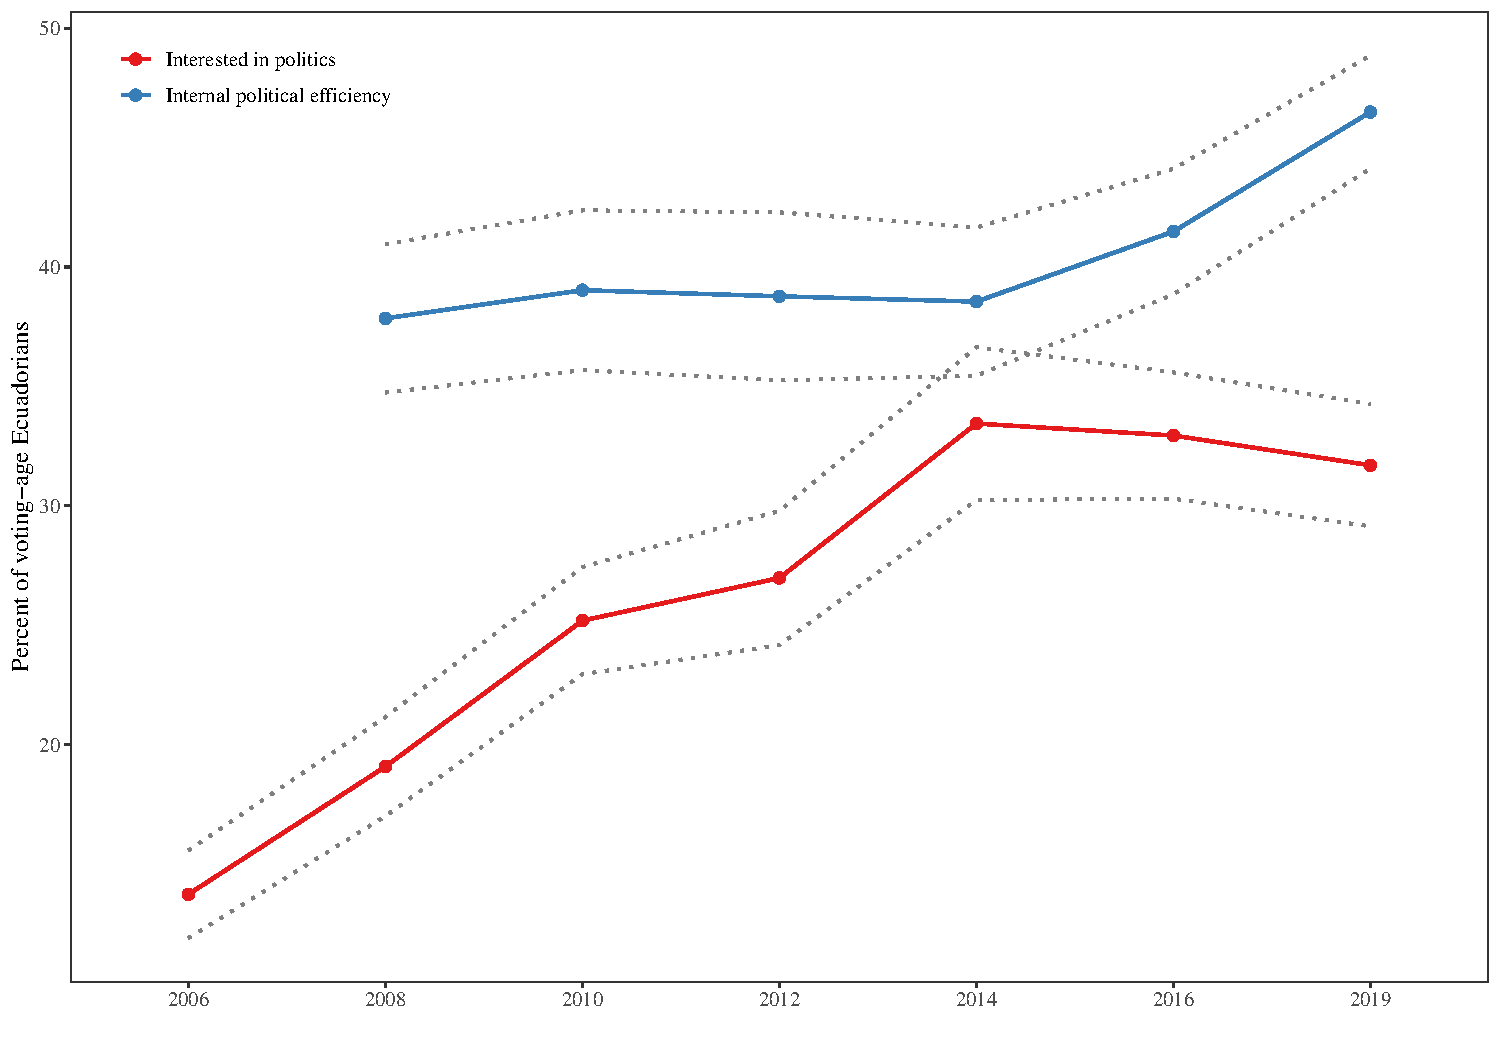
\includegraphics[width=\maxwidth]{figure/pol-int-graph-1} 

}


\end{knitrout}
\textbf{Note:} A time series of the internal political efficacy variable and the interest in politics variable. The internal political efficiency variable is dichotomized using the standard AB methodology as explained in \hyperref[app:first]{Appendix A}. Dotted lines represent the 95\% confidence intervals considering design effects. Data from the open-access AB databases. Figure prepared by the author.
\end{minipage}
}
\end{figure}

Figure \ref{fig:intpol} shows the percent who are interested in politics and also the percent who understand the country's politics. The gap between these two variables has increased from 2014 from 2016, and have a total historic correlation of 0.19. While they may appear to ask similar things, the two questions may imply different attitudes to politics: the political efficacy question simply asks if citizens are aware of politics and the second one asks if they're interested to enter the political scenario. It might be possible that, when separating these two questions, attitudes of apathy or pragmatism to the political society (understanding politics) are separated from an \enquote{idealist} attitude towards it of those who would like to enter politics.

A control for years of education is also added and it is significant, communicating that more educated respondents are less likely to justify corruption. Other things equal, an additional year of education is related to a 6 percentage points reduction in corruption tolerance. This finding is intuitive considering that more education may mean more knowledge about the costs of corruption. The social payoffs for being honest may be higher as also higher education may entail a better economic position which makes engaging in corrupt acts less economically attractive. 

Regarding the variables which measure corruption, it is possible to confirm findings by \textcite{Moscoso.2020}, \textcite{Lupu.2017} and \textcite{Singer.2016}: exposure to corrupt acts (paying or being asked to pay a bribe) is also strongly correlated with tolerance to them. A person who has been exposed to some form of bribing is about 15\% more likely to justify corruption according to the average partial effects in Table \ref{tab:apescomp}. The direction of causality is not clear in this case as it might be possible that a predisposed tolerance to corruption due to external factors makes citizens more likely to be in environments where corruption flourishes. \textcite{Moscoso.2018} finds that younger people and people with a higher number of children are more likely to be exposed to corruption with the 2016 Ecuador AB data. This may suggest that younger people justify corruption partly because they are more exposed by it: empirical models not shown explicitly show that an interaction term between age and corruption exposure is significant at the the 90\% confidence level. Corruption perceptions, on the other hand, play no role in determining corruption tolerance for this time period. This is also found by \textcite{Moscoso.2020} in 2019, however, \textcite{Lupu.2017} does find an effect of corruption perceptions on corruption tolerance for the whole Latin American region. An interaction term between year and corruption perceptions is not significant, although Figure \ref{fig:corrper} shows a significant increase of corruption perceptions between 2014 and 2016 (see \hyperref[app:first]{Appendix A}). 

% Make the corruption perceptions figure

\begin{figure}[htbp]
\fbox{
\begin{minipage}{\textwidth}
\caption{Corruption perceptions in Ecuador 2004-2016}
\label{fig:corrper}
\begin{knitrout}
\definecolor{shadecolor}{rgb}{0.969, 0.969, 0.969}\color{fgcolor}
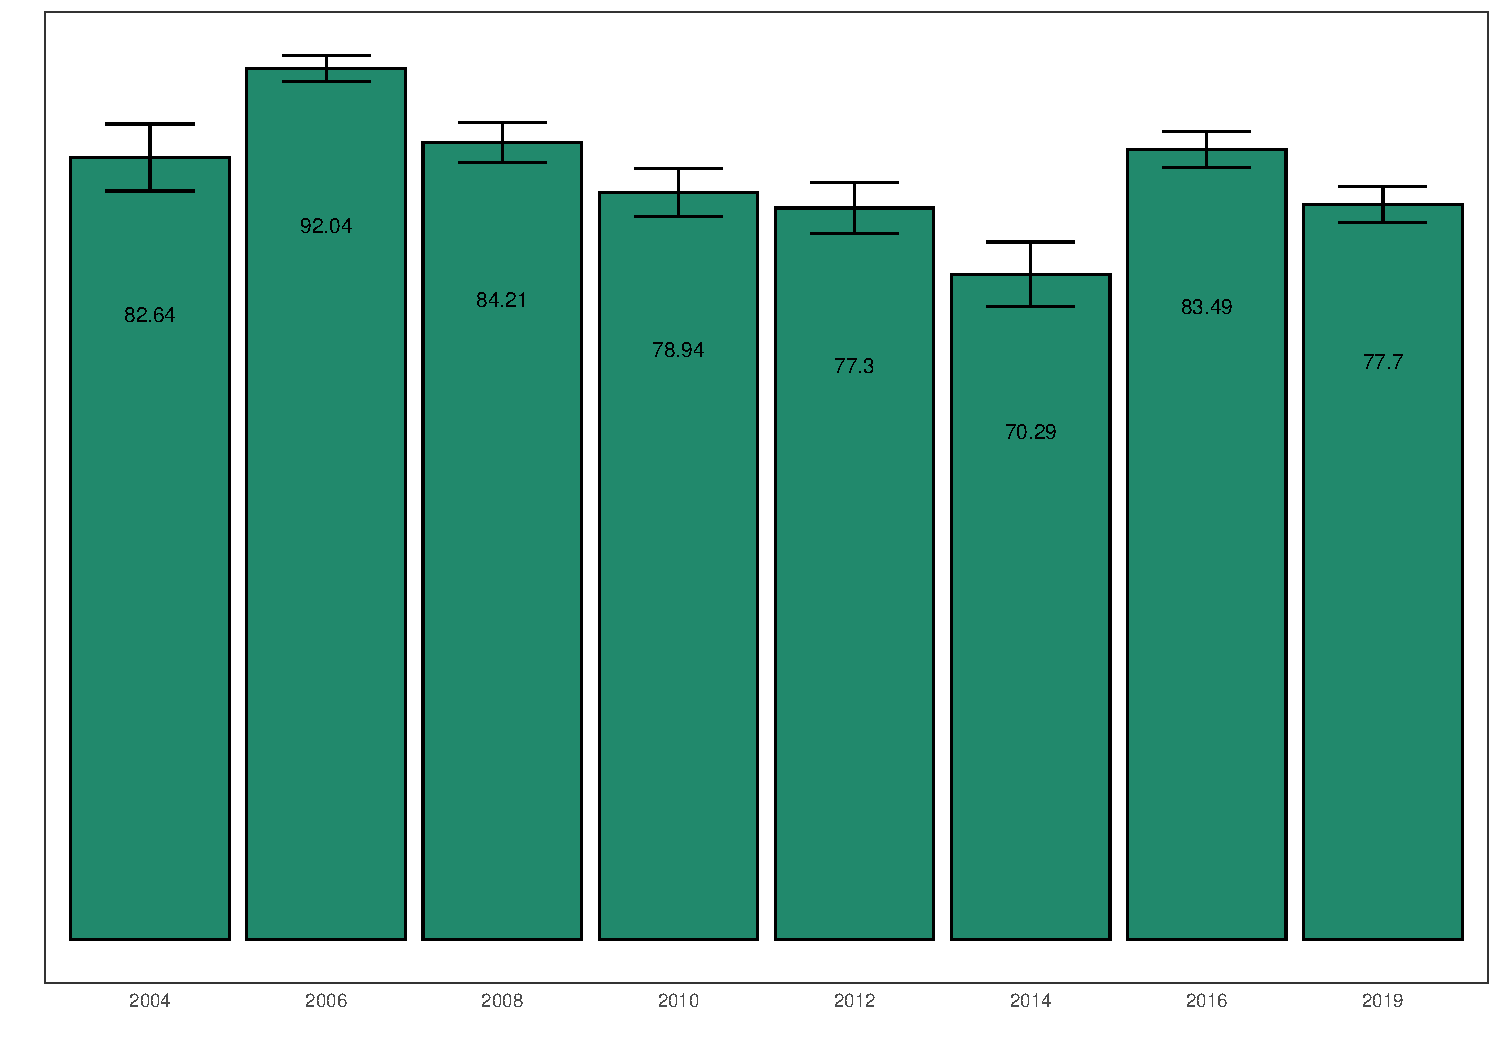
\includegraphics[width=\maxwidth]{figure/corrper_g-1} 
\end{knitrout}
\textbf{Note:} A time series of corruption perceptions in Ecuador. The corruption perceptions question was asked in a slightly different manner in 2016, thus the variable is recoded as explained in \hyperref[app:first]{Appendix A}, to construct this time series. Error bars represent the 95\% confidence intervals considering design effects. Data from the open-access AB databases. Figure prepared by the author.
\end{minipage}
}
\end{figure}

% Now the regressions which were not shown explicitly in text



A dummy variable equal to unity for respondents who have recently attended a protest is added and it is very significant. A person who has attended a protest is about 7\% more likely to justify corruption, other things equal. The reason why this happens might be related to a explanation of \textit{denial of victim} as proposed by \textcite{Ashforth.2003}. People who attend protests probably reject the current state of things, which may induce a feeling of contempt against society. They may believe dishonest acts could be justified in these adverse circumstances because they feel corrupt acts can be retribution to other dishonest acts done to them or by alleging that \textit{petty} corruption acts are nothing compared to grand corruption scandals. Since they have “declared” their rejection to the system in general, they have surrendered to its flaws and have no social incentives to remain honest.

Table \ref{tab:complexmod} also shows that after considering several variables suggested by the literature the interaction terms, as estimated in Table \ref{tab:simplemodel}, keep their sign and significance. Even after controlling for several important predictors of corruption tolerance, it is still true that unemployed people justified corruption more in 2014 but reduced their tolerance in 2016. People who approved the job performance of President Correa were less likely to justify corruption in both years, but their rejection of bribes was smaller in 2016. Finally, while the political identification was not important to predict corruption tolerance in 2014, it was significant in 2016; where people who identified as closer to the political right were more likely to justify corruption. To further explore the effects of these three key variables on corruption tolerance, cross-sectional models are estimated for 2014 and 2016 separately and shown below.



% Table of cross-sectional models
\begin{table}[htbp]
\begin{center}
\caption{Logit coefficients for cross-sectional models as seen in Equation \ref{eqn:crosssecmodel}}
\label{tab:crossmod}

\begin{tabular}[t]{lcc}
\toprule
  & Model 1 & Model 2\\
\midrule
Constant & \num{-0.006} & \num{-0.110}\\
 & (\num{0.663}) & (\num{0.479})\\
Woman & \num{0.059} & \num{0.141}\\
 & (\num{0.204}) & (\num{0.133})\\
Age & \num{-0.019}*** & \num{-0.029}***\\
 & (\num{0.007}) & (\num{0.004})\\
Years of education & \num{-0.030} & \num{-0.047}***\\
 & (\num{0.030}) & (\num{0.018})\\
Lives in urban setting & \num{0.151} & \num{-0.075}\\
 & (\num{0.238}) & (\num{0.152})\\
External political efficacy & \num{-0.032} & \num{-0.056}\\
 & (\num{0.054}) & (\num{0.039})\\
Internal political efficacy & \num{0.164}* & \num{0.077}*\\
 & (\num{0.097}) & (\num{0.045})\\
Participation in a protest & \num{0.436} & \num{0.205}\\
 & (\num{0.301}) & (\num{0.275})\\
Interest in politics & \num{-0.265} & \num{-0.253}*\\
 & (\num{0.227}) & (\num{0.136})\\
Perceptions of corruption & \num{-0.005} & \num{0.112}\\
 & (\num{0.207}) & (\num{0.175})\\
Exposure to corruption & \num{1.520}*** & \num{0.663}***\\
 & (\num{0.178}) & (\num{0.145})\\
Unemployment & \num{0.942}*** & \num{0.042}\\
 & (\num{0.236}) & (\num{0.164})\\
Approval of Pres. performance & \num{-0.533}*** & \num{0.025}\\
 & (\num{0.108}) & (\num{0.072})\\
Political wing & \num{-0.025} & \num{0.053}**\\
 & (\num{0.040}) & (\num{0.022})\\
\midrule
$N$ & \num{1039} & \num{1269}\\
AIC & \num{755.79} & \num{1434.40}\\
BIC & \num{832.75} & \num{1516.11}\\
Year & 2014 & 2016\\
\bottomrule
\end{tabular}


\end{center}
\textbf{Note:} Logit models for the cross-sectional models for 2014 and 2016 as seen in Equation \ref{eqn:crosssecmodel}. Data from the open-access AB databases. Standard errors consider design effects of the AB complex survey design.\\
*$p$ < 0.1, **$p$< 0.05, ***$p$ < 0.01.
\end{table}

% Table of Cross-Sectional APEs
\begin{table}[htbp]
\begin{center}
\caption{Average partial effects for cross-sectional models in Table \ref{tab:crossmod}}
\label{tab:apecross}

\begin{tabular}[t]{lcc}
\toprule
  & Model 1 & Model 2\\
\midrule
Age & \num{-0.002}*** & \num{-0.005}***\\
 & (\num{0.001}) & (\num{0.001})\\
Years of education & \num{-0.003} & \num{-0.009}***\\
 & (\num{0.003}) & (\num{0.003})\\
External political efficacy & \num{-0.003} & \num{-0.010}\\
 & (\num{0.006}) & (\num{0.007})\\
Internal political efficacy & \num{0.017}* & \num{0.014}*\\
 & (\num{0.010}) & (\num{0.008})\\
Interest in politics & \num{-0.028} & \num{-0.047}*\\
 & (\num{0.024}) & (\num{0.025})\\
Perceptions of corruption & \num{-0.001} & \num{0.021}\\
 & (\num{0.022}) & (\num{0.033})\\
Exposure to corruption & \num{0.161}*** & \num{0.124}***\\
 & (\num{0.019}) & (\num{0.027})\\
Unemployment & \num{0.100}*** & \num{0.008}\\
 & (\num{0.026}) & (\num{0.031})\\
Approval of Pres. performance & \num{-0.056}*** & \num{0.005}\\
 & (\num{0.012}) & (\num{0.013})\\
Political wing & \num{-0.003} & \num{0.010}**\\
 & (\num{0.004}) & (\num{0.004})\\
\midrule
$N$ & \num{1039} & \num{1269}\\
Year & 2014 & 2016\\
\bottomrule
\end{tabular}


\end{center}
\textbf{Note:} Average partial effects for logit cross-sectional empirical models in Table \ref{tab:crossmod}. Data from the open-access AB databases. Standard errors consider design effects of the AB complex survey design.\\
*$p$ < 0.1, **$p$< 0.05, ***$p$ < 0.01.
\end{table}

The coefficients shown in Table \ref{tab:crossmod} show that, while education is significant for the pooled regression, it is not for a 2014 cross-section: only in 2016 it is possible to detect a negative effect of education years in corruption tolerance. Table \ref{tab:apecross} shows that an additional year of education reduces the probability of justifying corruption by about 9 percentage points, all other things equal. A similar phenomenon is seen for the interest in politics variable: only in 2016 people who are interested in politics justify corruption more than those not interested. The exposure to corruption, internal political efficacy and age variables remain significant for both years. The effect of protest participation, while significant in the pooled regressions, is not significant in any of the individual years. 

The last rows of Table \ref{tab:crossmod} show the effects of the key regressors for 2014 ($\beta_{x^*}$ as defined in Equation \ref{eqn:crosssecmodel}). Model 1 shows that those who were unemployed justified corruption to a greater extent. However, as the interaction term in Table \ref{tab:crossmod} shows, the effect on unemployment for 2016 is smaller. The effect of unemployment or of any of the key regressors in 2016 can be understood as the \enquote{net} effect of the regressor as defined in Equation \ref{eqn:genmod}: $\beta_{x^*} + \delta_1 y_{16}$. In fact, according to the models in 2016 unemployed respondents do not display a different likelihood of justifying corruption relative to those who are not unemployed. The data shows that following the recession and loss of popularity of the regime, the unemployed remained approximately equal in their corruption tolerance proclivities relative to those who were not unemployed.

It is possible that initially unemployed people justified corruption more because it was their “steady state” of corruption tolerance: unemployed people are economically disadvantaged which gives them incentives to engage in corrupt actions which yield positive economic payoffs. Additionally, as they are unable to enter the job market for some time, they might feel more alienated from society, which might decrease social or moral incentives to remain honest by renouncing the economic payoffs that corruption may offer, as it has been explained previously. The change in corruption tolerance behavior for 2016 is more difficult to understand. It is possible that since the recession many lost their jobs and they have had relatively short unemployment spells. The recently unemployed may not feel too alienated from society and thus have not adopted an attitude of pragmatism toward the current circumstances. Savings or family income may support the recently unemployed which makes them feel less desperate and prone to take the “moral high ground”. This
all contributes to them still feeling part of society, which reduces their rationalization of corruption. However, with larger unemployment spells, desperation may trigger more pragmatic points of view, which will lead to higher corruption tolerance in future years. All of this contributes to the effect of unemployment in 2016 not being statistically different from zero, as seen in Table \ref{tab:crossmod}.

To better understand the implications of the political variables' coefficients and their change in time, consider a key actor on corruption normalization, leadership. Having initially branded himself as \enquote{the biblical underdog} \parencite[para. 4]{Hedgecoe.2009}, President Correa distanced himself from the country's political elite and constantly denounced  corruption and injustice in the system. The new government promised a radical change when it started its tenure in 2007 and did deliver as it gave Ecuador a politically stable though totalitarian environment, as well as other changes in political and economical mechanisms \parencite{Weisbrot.2017}. The President had explicitly stated that he would battle corruption and fiscal evasion \enquote{to the death} \parencite{Ortiz.2013}. Thus, supporters of this regime had higher social sanctions if they engaged in or justified corrupt behavior, as this may have implied that the economic and political model they supported was flawed.

However, by 2016 the popularity of the regime faced a sharp decrease. Several narratives started to be constructed by President Correa and his officials to explain the flaws and weaknesses that opponents had denounced. These included reducing corruption accusations to \enquote{political persecution} or unfounded claims done because of upcoming elections \parencite{Melendez.2017}. A statement by the President represents a particularly relevant example: a regime-affiliated newspaper portrayed how Correa qualifies the Panama Papers as a \textit{selective fight against corruption} which is nothing but another kind of corruption, as well as a \textit{strategy by power groups} to destabilize democratically-elect governments \parencite[para. 5-7]{Telegrafo.2016}. 

Even as corruption accusations had planted the seed of a deep investigation about a complex corruption scheme involving top government officials and large corporations \parencite{Villavicencio.2019}, authorities within the Correa administration reduced the importance of these events, which created a narrative for regime supporters. If the legitimacy of those who denounce and control corruption is questioned by an important authority of the organization, corrupt acts can be more easily normalized \parencite{Ashforth.2003}. Thus, if there was a greater incidence of corrupt acts as well as numerous attempts by the authorities to justify them, it can be understood how supporters of the regime started to justify corruption more.

The data also show how people who identify with the political right became more corruption-tolerant in 2016. It is not clear if there is a causal relationship involving the political right and corruption tolerance. This is because it has been determined that in Ecuador the answer to the political identification question has little to do with the traditional principles of the political wings that are commonly understood. Rather, it is possible that the political self-identification of Ecuadorians follows a multidimensional perspective \parencite{Moncagatta.2020b}, not too accurately measured with an indicator like the one used here. 

A potential explanation to the sign on this variable is that those who identify with the right do so partially because they consider themselves to be against the government in place. This is reasonable considering the increase in the percentage of "rightists" between 2014 and 2016, which moves together with regime's downfall. Additionally, it is possible that anti-regime attitudes formed under a common set of ideas rather than under a political party or figure, since during President Correa's tenure opposition forces did not materialize strongly behind a party or leader \parencite{Melendez.2017}. It is sensible to believe that no political wing has any particular preference for justifying or rejecting corruption, as important actors in both political wings have spoken against it, academics \parencite{Holcombe.2015} and politicians \parencite{Morris.2021} alike. However, anti-regime respondents rather than \enquote{rightists} might rationalize corruption as a form of revenge, as proposed by \textcite{Ashforth.2003} and noted by \textcite{Adoum.2000}.






\end{document}
